\documentclass[a4paper,11pt,openright]{report}

%%%%%%%%%%%%%%%%%%%%%%%%%%%%%%%%%%%%%%%%%%%%
\usepackage[utf8]{inputenc}
%\usepackage[latin1]{inputenc}
\usepackage[T1]{fontenc}
\usepackage{url}           % definit les commandes \url et \path
%\usepackage[normalem]{ulem}
\usepackage{fancyhdr} %entete
\usepackage{lastpage}
\usepackage{titlesec}
\usepackage{geometry} %figure
\usepackage{times}
\usepackage{amsmath}
\usepackage{graphicx}      % permet inclusion de figures
\usepackage{pdfpages} %permet integrer doc html
\usepackage{ae}            
\usepackage{bm}
\usepackage{xcolor}
\usepackage{epsf}
\usepackage{tikz}
%\usepackage{frenchle}
\usepackage[french]{babel} %pour un document en français
\usepackage[Sonny]{fncychap} % pour format chapitre
\usepackage{enumitem}
%\userpackage{titlesec}
\usepackage{listings}%pour insérer du code source
\usepackage{hyperref}%rend actif les liens, références croisées, toc…
%%%%%%%%%%%%%%%%%%%%%%%%%%%%%%%%%%%%%%%%%%%%
\geometry{hmargin = 2.5 cm, vmargin = 3.0 cm} % c'est pas bien...vmargin = 3 mieux !!!
\setcounter{secnumdepth}{3} % pour la numerotation dans le corps du document
\setcounter{tocdepth}{3}    % pour l'apparition dans la table des matieres
\newcommand{\HRule}{\rule{\linewidth}{0.5mm}}
\fancyhead[R]{}
\fancyfoot[C]{\thepage/\pageref{LastPage}}
\hypersetup{
    colorlinks=true, % Pour des liens colorés au lieu de cadres
    linkcolor=black,  % Couleur des liens internes (par défaut: rouge)
    urlcolor=blue,   % Couleur des liens URL (par défaut: cyan)
}
%%%%%%%%%%%%%%%%%%%%%%%%%%%%%%%%%%%%%%%%%%%%



\begin{document}
%%%%%%%%%%%%%%%%%%%%%%%%%%%%%%%%%%%%%%%%%%%%
\begin{titlepage}
\begin{center}
\textsc{\LARGE M2-BBS UNIVERSITÉ PAUL SABATIER} \\
%%%%%%%%%%%%%%%%%%%%%%%%%%%%%%%%%%%%%%%%%%%%
  \begin{figure}[htbp] 
  \begin{center}
  
\includegraphics[width=8cm]{Logo_UT3.jpg}    
  \label{fig:logoUPS}
  \end{center}
  \end{figure} 
%%%%%%%%%%%%%%%%%%%%%%%%%%%%%%%%%%%%%%%%%%%% 
\vspace{2cm}
\textsc{\Large Rapport - GDNS - Application post-génomique}\\[0.5cm]

\HRule \\[0.5cm]
{\Huge \bfseries Caractérisation d'un ensemble de gènes\\[0.3cm] 
 via la création d'une application Python et  d'une base de données Neo4j \\[0.3cm]
- set.M2.6.txt -}\\[0.3cm] 
{\normalsize \textit{version corrigée}}\\[0.4cm]
\HRule\\[1cm]

\url{https://github.com/boumbo85/ecoli-neo4j-genomics}
\vspace{1cm}

\begin{minipage}{0.4\textwidth}
\begin{flushleft} \large
\emph{Auteure : }\\
Julie \textsc{CAMPOS} 
\end{flushleft}
\end{minipage}
\begin{minipage}{0.4\textwidth}
\begin{flushright} \large
\emph{Sous la supervision de : } \\
Dr. Roland \textsc{BARRIOT}
\end{flushright}
\end{minipage}

\begin{tikzpicture}[remember picture, overlay]
 \begin{scope}[shift={(current page.south west)},shift={(2.5,2)},scale=1]
 \shade[ball color=blue,opacity=.6] (0,0) circle (10ex);
 \shade[ball color=blue,opacity=.8] (1.7,1) circle (5ex);
 \shade[ball color=blue,opacity=.8] (1.5,3) circle (2ex);
 \shade[ball color=blue,opacity=.5] (-0.5,3) circle (1ex);
 \shade[ball color=blue,opacity=.8] (1,4) circle (1ex);
 \shade[ball color=blue,opacity=.6] (3.5,2.5) circle (2ex);
 \shade[ball color=blue,opacity=.8] (2.5,4.5) circle (4ex);
 \shade[ball color=blue,opacity=.5] (3,4) circle (3ex);
 \shade[ball color=blue,opacity=.8] (4.5,4.5) circle (3ex);
 \shade[ball color=blue,opacity=.5] (5.1,4.7) circle (2ex);
 \shade[ball color=blue,opacity=.8] (5,6) circle (1.5ex);
 \shade[ball color=blue,opacity=.6] (3.5,5.5) circle (2ex);
 \shade[ball color=blue,opacity=.8] (5,3) circle (1ex);
 \end{scope}
\end{tikzpicture}

\vfill
{\large Novembre 2023}

\end{center}
\end{titlepage}
%%%%%%%%%%%%%%%%%%%%%%%%%%%%%%%%%%%%%%%%%%%%




%%%%%%%%%%%%%%%%%%%%%%%%%%%%%%%%%%%%%%%%%%%%
\newpage
\pagestyle{empty}
%\maketitle                    
\tableofcontents
%%%%%%%%%%%%%%%%%%%%%%%%%%%%%%%%%%%%%%%%%%%%




%%%%%%%%%%%%%%%%%%%%%%%%%%%%%%%%%%%%%%%%%%%%
\chapter{INTRODUCTION}
\thispagestyle{empty}
\clearpage
\newpage
\setcounter{page}{1} %pour forcer la numérotation à commencer à cette page
\pagestyle{fancy}

\textbf{Préambule :} Nous choisissons d'écrire le rapport en français et les codes (R, Phyton) en anglais.

	\section{CONTEXTE}
Les recherches en génomique ont permis de réaliser des progrès considérables dans l’élaboration de cartes physiques et
génétiques et de déterminer la séquence de nombreux génomes. Elles ont ouvert la voie et grandement contribué à l’acquisition de nouvelles connaissances en physiologie par exemple. Parallèlement, le développement de nouvelles technologies d’analyses moléculaires à grande échelle (métagénomique, transcriptomique et protéomique) et l’essor de la bio-informatique rendent maintenant possible l’exploitation de ce flux de données et permettent par une étude globale de l’expression des gènes d’avoir
une vision moins réductionniste du vivant. Ces progrès sont à l’origine d’une nouvelle discipline de la génomique appelée la "post-génomique" (ou génomique fonctionnelle).  Elle vise à comprendre la fonction et la régulation de tous les gènes et protéines qui conditionnent le fonctionnement de l’organisme.\\
De nombreuses expériences de laboratoire requièrent une étape de séquençage d'échantillons (séquences nucléotidiques) et permettent ainsi de mettre en évidence une liste de gènes d'intérêts. Ces séquences sont obtenues par des expériences telles que : RNAseq, sRNAseq, CHIP-sep ou ATACseq.  L'étape d'après consiste  à interpréter et caractériser cette liste de gènes. C'est ici que la "post-génomique" entre en jeu. La "post-génomique" fait référence à la recherche et l'analyse en génomique survenant après le séquençage d'échantillons d'ADN ou d'ARN. Elle englobe divers domaines de recherches, notamment :

\begin{itemize}
	\item \textbf{analyse fonctionnelle de gènes} 
	\item \textbf{protéomique} 
	\item \textbf{structure 3D des protéines} 
	\item \textbf{épigénomique} 
	\item \textbf{analyse des réseaux biologiques} 
	\item \textbf{transcriptomique} 
	\item \textbf{expression génique} 
	\item \textbf{métagénomique} 
	\item \textbf{évolution moléculaire} 
\end{itemize}

C'est donc un enjeu majeur que de savoir caractériser une liste de gènes afin d’interpréter les résultats.

	\section{OBJECTIF}
Cette étude vise donc à caractériser un ensemble de gènes, à partir d'une liste fournie d'identifiants  (\textit{bnumber}) de gènes (set.M2.6.txt). Nous répondrons entre autre à la question suivante :
A quels processus biologiques, fonctions moléculaires ou localisations sub-cellulaires peut-on les relier ? \\
 A travers cet exemple, l'objectif intrinsèque est d'implémenter une base de données non structurées (graphe, Neo4j) incluant toutes les informations relatives à un projet (par exemple les références "PubMed", nom des gènes, fonctions biologiques, voies métaboliques), et d'explorer ses nombreuses possibilités.  

	\section{MÉTHODE}
Nous présenterons ici une méthode pour étudier cette liste de gènes, s'appuyant sur la construction d'une base de données sous forme de graphe (\textbf{"Neo4j"}), et la création d'une application python permettant d'automatiser cette caractérisation. L'application prendra en entrée une liste de gènes d’intérêt (appelée \textit{"query"}), ainsi qu'une liste de gènes de référence (appelée \textit{"target"}). L'application retournera en sortie des statistiques descriptives, une liste de termes en fonction de l'option choisie (mots clef de fonctions biologiques, identifiants "GOTerms", références "Pubmed", voies métaboliques). Il s'agit d'une approche par ensembles d'enrichissement. Le but de cette méthode est de déterminer si les gènes interrogés (requête) présentent un  enrichissement significatif dans certaines fonctions biologiques par rapport à ce qui serait attendu de manière aléatoire
\footnote{Nous suivrons la méthode proposée en travaux pratiques{\url {https://silico.biotoul.fr/enseignement/m2bbs/gdns-ap/GDNS-APG.Mise.en.oeuvre.html\#approche-par-ensembles-enrichissement}}}. 
%%%%%%%%%%%%%%%%%%%%%%%%%%%%%%%%%%%%%%%%%%%%






%%%%%%%%%%%%%%%%%%%%%%%%%%%%%%%%%%%%%%%%%%%%
\chapter{CREATION DE LA BASE DE DONNÉES NEO4J}
\thispagestyle{empty}
\clearpage
\newpage
Les script R pour l'intégration de la base de néo4j ont été élaboré conjointement avec Claire DELAMARE-DEBOUTTEVILLE.

	\section{PRÉSENTATION DES DONNÉES}
L'échantillon d'étude est issu de la bactérie \textbf{\textit{Escherichia.coli}}(\textit{E.coli}), souche \textbf{K-12 MG1655} (Ecocyc). La souche K-12 MG1655 est une souche très répandue en laboratoire
\footnote{url{https://www.ncbi.nlm.nih.gov/Taxonomy/Browser/wwwtax.cgi?id=511145}, \url{https://www.ncbi.nlm.nih.gov/pmc/articles/PMC9997739/}}. 
\textit{E.coli} est une entérobactérie, de type gram négatif. Elle est présente dans la flore intestinale des organismes homéothermes \footnote{url{https://fr.wikipedia.org/wiki/Escherichia$\_$coli}}. E.coli participe à la suppression de la croissance des bactéries nocives et  synthétise des vitamines dans le tractus intestinal. La plupart des souches d'\textit{E.coli} sont sont commensales, mais une minorité de souches peut provoquer des maladies chez l'homme. \\  

E.\textit{coli} possède un génome à ADN double brin circulaire de 4,6 millions de paires de bases, 4401 gènes (Uniprot)
\footnote{url{https://pubmed.ncbi.nlm.nih.gov/11574054/}}.

%%%%%%%%%%%%%%%%%%%%%%%%%%%%%%%%%%%%%%%%%%%%
	\begin{figure}[htbp] 
    \begin{center}
    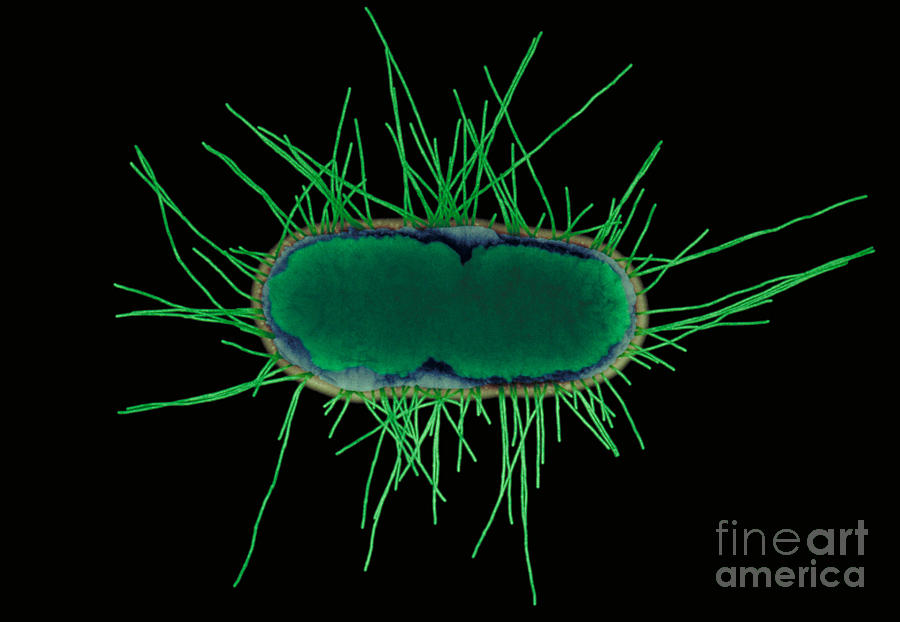
\includegraphics[width=16cm]{ecoli.png}   
    \caption{Micrographie électronique à transmission (TEM) en couleur d'\textit{Escherichia Coli} K12 - 2014 - by Kwangshin Kim}  
    \label{fig:pict}
    \end{center}
    \end{figure}
%%%%%%%%%%%%%%%%%%%%%%%%%%%%%%%%%%%%%%%%%%%%



Nous travaillerons sur deux listes de gènes, une de test (set1)dont les résultats sont connus, pour mettre en place l'application , et la liste d'étude (set.M2.6, cf.~\ref{annexe:Q6}) à analyser. \\ Nous utiliserons comme génome de référence GCF$\_$000005845.2, au format \textcolor{orange}{.gbff} \\
(fichier \textcolor{violet}{GCF$\_$000005845.2.gbff.gz}).

	\section{MODÉLISATION DE LA BASE DE DONNÉES}
L'implémentation de la base de donnée \textbf{"Neo4j"} requière la création de nœuds et de relations (connexions entre les nœuds).  Nous intégrerons dans la base de données entant que nœuds, les informations suivantes  \footnote{url {https://silico.biotoul.fr/enseignement/m2bbs/gdns-ap/GDNS-APG.Mise.en.oeuvre.html$\#$approche-par-ensembles-enrichissement} partie 1.3} :
\begin{itemize}
	\item \textbf{Gene : } identifiants (\textit{"bnumber"},nom des gènes, sens du brin (\textit{"strand"}) ainsi que leur position sur le(s) chromosome(s)
	\item \textbf{Alias : } les alias/synonymes des noms de gènes
    \item \textbf{Keyword : }  identifiants \textit{"Uniprot"} et mots clef de fonctions biologiques (\textit{UniProt Proteome dataBase})
    \item \textbf{InterPro : } identifiants \textit{"Uniprot"} et nom des domaines protéiques (\textit{UniProt Proteome dataBase})
    \item \textbf{PubMed : } identifiants \textit{"PubMed"} et nom des références bibliographiques (GenBank/RefSeq) 
    \item \textbf{TU : } identifiants \textit{"Ecocyc"}, nom, sens du brin, position de début et fin des unités de transcription. Pour rappel, une unité de transciption est une région du génome transcrit en ARN. Certains gènes peuvent coder pour plusieurs protéines (un isoforme = une unité de transcription)    
    \item \textbf{Pathway : } identifiants \textit{"Ecocyc"}, nom  des voies métaboliques 
    \item \textbf{GOTerm : } identifiants \textit{"GOTerm"}, nom  et description des termes de l’ontologie des gènes (\textit{Gene Ontology} + \textit{UniProt}) 
    \item \textbf{StringDB : } Scores d'association entre paires de gènes/protéines basés sur la co-expression, le lien phylogénomique, et les interactions protéine-protéine. 
\end{itemize}

\textbf{Remarques : } 
\begin{enumerate}
\item Chaque nœud contient un identifiant unique (clef primaire). Donc chaque nœud correspond à une liste de termes uniques.
\item Selon les sources de données, les méthodes de référencement et d’identification peuvent ne pas être les mêmes. Dans cette étude, nous nous baserons sur les \textit{bnumbers}(identifiant Uniprot). Le jeu sera d'associer à chaque identifiant du nœud, un \textit{bnumbers}
\end{enumerate}

Les relations entre les nœuds sont décrites d'après le schéma suivant : (\textit{cf. fig.\ref{fig:model}})\\

%%%%%%%%%%%%%%%%%%%%%%%%%%%%%%%%%%%%%%%%%%%%
	\begin{figure}[htbp] 
    \begin{center}
    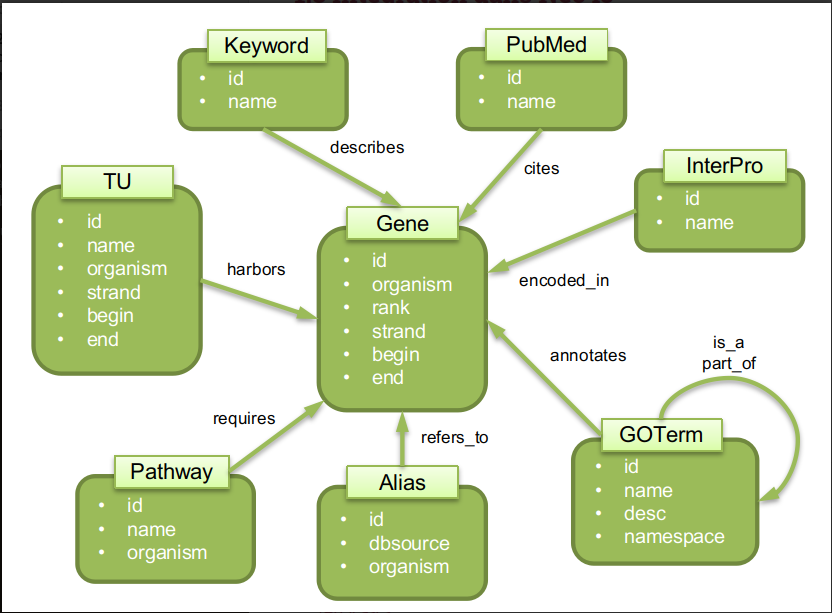
\includegraphics[width=16cm]{modelBD.png}   
    \caption{Modélisation de la base de données Neo4j}  
    \label{fig:model}
    \end{center}
    \end{figure}
%%%%%%%%%%%%%%%%%%%%%%%%%%%%%%%%%%%%%%%%%%%%

Les relations sont construites de tel sorte qu'il existe au minimum deux attributs : l'identifiant du nœud concerné et le \textit{"bnumber"} associé. Chaque relation est donc constituée d'une liste unique d'associations \textbf{terme - \textit{bnumber}}.

\section{PRÉREQUIS}
Pour le projet, nous avons utilisé les outils informatiques et leur versions associées suivantes 
\footnote{Pour plus de détails, cf. les fichiers "requirements" dans le github du projet : https://github.com/boumbo85/ECOLI} :

\begin{itemize}
\item \textbf{Système d'exploitation (OS) : } Linux FEDORA $\rightarrow$  version release 37 (Thirty Seven)
\footnote{\textcolor{green}{lsb$\_$release -a}}

\item \textbf{Logiciels : } 
	\begin{itemize}[label=\textbullet]
	\item \textbf{conda : }  $\rightarrow$  version (23.3.1)
	\item \textbf{Neo4j Desktop : }  $\rightarrow$  version (1.4.15)
	\item \textbf{Neo4j : } $\rightarrow$ version (4.4.9) (\textit{Edition: community})
	\item \textbf{R base : }  $\rightarrow$ version (4.3.2)
	\item \textbf{Rstudio : } $\rightarrow$ version (2023.06.1 524) - "Mountain Hydrangea"
	\begin{verbatim}
	Release (547dcf861cac0253a8abb52c135e44e02ba407a1, 2023-07-08) 
	for Fedora release 37 (Thirty Seven) 
	Mozilla/5.0 (X11; Linux x86_64) AppleWebKit/537.36 (KHTML, like Gecko) 
	QtWebEngine/5.15.12 Chrome/87.0.4280.144 Safari/537.36
	\end{verbatim}
	\item \textbf{Python : } $\rightarrow$ version (3.12.0) 
	\item \textbf{VScode : } $\rightarrow$ version (1.83.1)
	\end{itemize}
	
\item \textbf{Package Python (3.12.0) : } 
	\begin{itemize}[label=\textbullet]
	\item pandas  $\rightarrow$  version (2.1.2)
	\item numpy $\rightarrow$ version (1.26.1) 
	\item monotonic $\rightarrow$ version (1.6)
	\item py2neo $\rightarrow$ version (2021.2.4)
	\item neo4j $\rightarrow$ version (5.14.0)
	\item scipy $\rightarrow$ version (1.11.3)
	\item matplotlib $\rightarrow$ version (3.8.1)
	\item argparse (parso $\rightarrow$ version 0.8.3)
	\end{itemize}

\item \textbf{Package R (4.3.2) : } 
	\begin{itemize}[label=\textbullet]
	\item tidyverse (CRAN)  $\rightarrow$  version (2.1.2)
	\item tibble (CRAN)  $\rightarrow$  version (3.2.1)
	\item dplyr (CRAN)  $\rightarrow$  version (1.1.3)
	\item jsonlite (CRAN) $\rightarrow$  version (1.8.7)
	\item RMySQL (CRAN) $\rightarrow$ version (6.1.11) 
	\item neo4r (CRAN)$\rightarrow$ version (0.1.1)
	\item reticulate (CRAN) $\rightarrow$ version (1.34.0)
	\item STRINGdb (BioConductor) $\rightarrow$ version (2.12.0)
	\item igraph $\rightarrow$ version (1.5.1)
	\end{itemize}

\end{itemize} 

	\section{PRÉPARATION DES DONNÉES} 
\textit{(cf. ANNEXE~\ref{annexe:R1} et }
\url{https://silico.biotoul.fr/enseignement/m2bbs/gdns-ap/GDNS-APG.Mise.en.oeuvre.html\#approche-par-ensembles-enrichissement} \\
Le but ici est de créer un fichier au format \textcolor{orange}{.csv} par nœud et par relation. Chaque nœud est une liste unique de termes (selon les catégories d'informations retenues (Goterm, Keywords, Uniprot..). Chaque terme est associé à un identifiant unique (clef primaire) et une sélection d'informations relatives à cet identifiant. Chaque relation est une liste d'association unique de \textbf{\textit{"bnumber"}} et termes. Voici comment nous construisons les fichiers \textcolor{orange}{.csv}. \\ 

Nous récupérons le protéome d'\textit{Escherichia.coli} K12 MG1655, au format \textcolor{orange}{.tsv} sur le site d'Uniprot \footnote{\url{https://www.uniprot.org/}}.  Nous choisissons comme référence de notation les \textit{"bnumber"}. A partir de ce fichier, nous pouvons extraire les listes de :
\begin{itemize}
	\item \textbf{\textit{"bnumber"} : } à partir de la colonne "Gene Names (ordered locus)" (liste des identifiants selon plusieurs système de notations): \\ 
	\textcolor{blue}{4401 lignes (uniques)}
	\item \textbf{Goterm : } à partir de la colonne "Gene Ontology IDs" (liste des Goterms) : \\ 
	\textcolor{blue}{22430  lignes (uniques)}
	\item \textbf{Keywords} à partir de la colonne "Keywords" (liste des mots clef des fonctions biologiques) : \\
	\textcolor{blue}{27506 lignes (uniques)}
	\item \textbf{InterPro} à partir de la colonne "InterPro" (liste des identifiants InterPro correspondant à un domaine/motif structural):\\
	\textcolor{blue}{15636  lignes (uniques)}
\end{itemize}   

associées à chaque nom de gène. Nous obtenons une liste d'association unique de \textit{"bnumber"} et de terme (\textbf{Keywords}, \textbf{InterPro} et \textbf{Goterm}).

Les unités de transcription (\textbf{TU})\footnote{\url{https://www.ecocyc.org/group?id=biocyc17-55140-3842483291}}
 et les voies métaboliques (\textbf{Pathway})\footnote{\url{https://www.ecocyc.org/group?id=biocyc17-55140-3842483872}}
  sont disponibles sur le site d'Ecocyc (\url{https://www.ecocyc.org/}). Cette fois-ci, nous devons faire correspondre l'identifiant "Ecocyc" avec l'identifiant "Uniprot", les \textit{"bunmber"}. Nous trouvons cette correspondance dans la table "gènes"\footnote{\url{https://www.ecocyc.org/group?id=biocyc13-55140-3842501533}}.

Les identifiants \textbf{PubMed} sont extrait via une application python fournie. \\


\section{INTÉGRATION DES DONNÉES DANS LA BASE}
\textit{(cf. ANNEXE\ref{annexe:R2}}
	\subsection{MÉTHODE}
Nous utilisons une image docker de Neo4j(neo4j:4.4.9-community) pour se connecter avec "podman" (linux Fedora), avec la commande \textcolor{violet}{"BASH"} suivante : \\
\textcolor{green}{podman pull neo4j:4.4.9-community} \\
\\ Cela permet d'utiliser la version de Neoj que l'on souhaite et évite d'installer Neo4j Desktop. Il s'agit maintenant  de connecter le docker avec notre session locale, avec la commande \textcolor{violet}{"BASH"} suivante : \\
\textcolor{green}{podman run --rm -it --name neo4j \ \\
   -p 7474:7474 \ \\
   -p 7687:7687 \ \\
   -v ./neo4j.data:/data \ \\
   -v ./neo4j.import:/import \ \\
   -e NEO4J$\_$AUTH=neo4j/omybioinfo \ \\
      --user="\$(id -u):\$(id -g)" \ \\
   neo4j:4.4.9-communit} \\
La base de donnée implémentée avec succès se présente donc ainsi : (\textit{cf. fig.\ref{fig:BDfull}})\\

%%%%%%%%%%%%%%%%%%%%%%%%%%%%%%%%%%%%%%%%%%%%
	\begin{figure}[htbp] 
    \begin{center}
    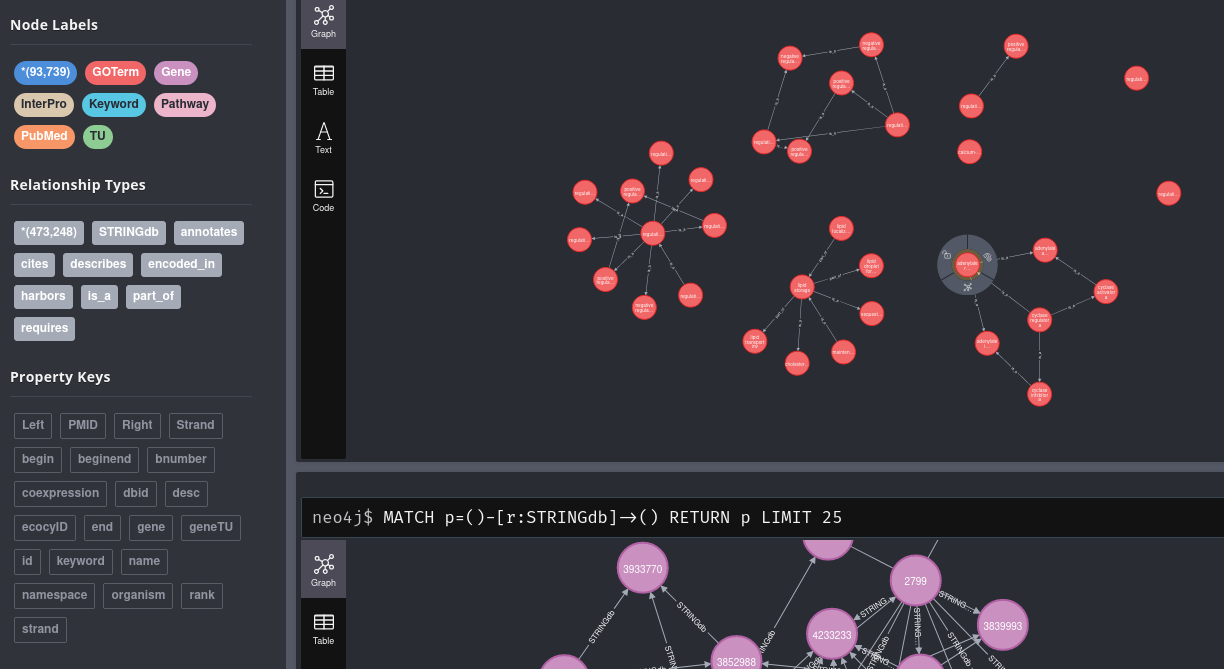
\includegraphics[width=16cm]{BD.png}   
    \caption{Aperçu de la base de donnée Neo4j }  
    \label{fig:BDfull}
    \end{center}
    \end{figure}
%%%%%%%%%%%%%%%%%%%%%%%%%%%%%%%%%%%%%%%%%%%%


\subsection{DESCRIPTION}
La base de données contient , incluant :
\begin{itemize}
\item \textbf{7 nœuds} tels que :
	\begin{itemize}[label=\textbullet]
	\item 4 315 "\textbf{Genes}"
	\item 385 "\textbf{Keywords}"
	\item 6 760 "\textbf{InterPros}"
	\item 42 887 "\textbf{GOTerms}"
	\item 3 634 "\textbf{TUs} "
	\item 438 "\textbf{Pathways}"
	\item 35 320 "\textbf{PubMeds}"
	\end{itemize}
	
\item \textbf{9 relations } telles que :
	\begin{itemize}[label=\textbullet]
	\item 27 323 "\textbf{describes}" (relation "\textbf{Keyword}" $\rightarrow$ "\textbf{Gene}"
	\item 101 841 "\textbf{cites} " (relation "\textbf{PubMed}" $\rightarrow$ "\textbf{Gene}"
	\item 15 515 "\textbf{encoded$\_$in}" (relation "\textbf{InterPro}" $\rightarrow$ "\textbf{Gene}"
	\item 68 521 "\textbf{is$\_$a}" (relation "\textbf{GOTerm}" $\rightarrow$ "\textbf{GOTerm}"
	\item 6 785 "\textbf{part$\_$of}" (relation "\textbf{GOTerm}" $\rightarrow$ "\textbf{GoTerm}"
	\item 22 373 "\textbf{annotates}" (relation "\textbf{GOTerm}" $\rightarrow$ "\textbf{Gene}"
	\item 6 170 "\textbf{harbors}" (relation "\textbf{TU}" $\rightarrow$ "\textbf{Gene}"
	\item 2 747 "\textbf{requires}" (relation "\textbf{Pathway}" $\rightarrow$ "\textbf{Gene}"
	\item 378 893 "\textbf{STRINGdb}" (gènes co-exprimés)
	\end{itemize}
	
\end{itemize}
%%%%%%%%%%%%%%%%%%%%%%%%%%%%%%%%%%%%%%%%%%%%




%%%%%%%%%%%%%%%%%%%%%%%%%%%%%%%%%%%%%%%%%%%%
\chapter{APPROCHE PAR ENSEMBLE : ENRICHISSEMENT}
\thispagestyle{empty}
\clearpage
\newpage

	\section{CRÉATION DE L'APPLICATION PYTHON}
		\subsection{Description}
Le script python de l'application d’enrichissement a été élaboré conjointement avec Claire DELAMARE-DEBOUTTEVILLE. \textit{(cf.~ANNEXE~\ref{annexe:app}}) et le fichier \textcolor{blue}{'app.py'}. \\
Le script d’enrichissement prend en entrée un ensemble de gènes requêtes (ici le "set 6"). Le "set 6" est une liste d'identifiant de gènes \textbf{\textit{"bnumber"}}. Le format de la liste du "set 6" a besoin d'être transformée afin d'être conforme au format d'entrée de notre application. En effet, la liste "set 6" contient un identifiant par ligne. Or il faudrait que les identifiants soient séparés d'un espace standard et non d'un saut de ligne (modification via la commande \textcolor{violet}{"BASH"} : \textcolor{green}{tr -s '/n' ' ' < query6 > query6.txt}). Le script permet de :
\begin{itemize}
	\item se connecter à la base de données Neo4j (BD) nouvellement créée
	\item d'interroger celle-ci via des requêtes \textcolor{violet}{"CYPHER"} : récupérer les termes/mot clefs associés à la liste de \textbf{\textit{"bnumber"}} de gène de l'ensemble requête.
	\item réaliser une analyse univariée  (statistiques descriptives) sur la liste de gènes inconnus et les mots clefs collectés
	\item comparer l'ensemble de termes requêtes (\textit{"query"}) avec l'ensemble de terme de référence (\textit{"target"}) pour identifier les éléments en commun ('coverage')
	\item réaliser des tests statistiques avec plusieurs méthodes (binomiale, hypergéométrique, test du $\chi^2$) sur chacun des termes (p-valeur ajustée aux multi tests ou non) afin de déterminer si cette différence est statistiquement due au hasard ou non (mesure de dissimilarité)
\end{itemize}

\subsubsection{Principe étape des tests statistiques : }
Nous chercherons à savoir si les différences observées entre l'ensemble requête et de référence sont statistiquement significatifs. Pour cela, nous suivrons les étapes classiques dans l'exécution de tests statistiques :
\begin{enumerate}
\item Définir les hypothèses de départ H0 (nulle) et H1 (alternative) 
\item Choisir un test statistique pour contrôler H0
\item Définir la distribution de la statistique sous l’hypothèse H0 (est réalisée)
\item Fixer valeur seuil alpha (5\%)
\item Calculer les probabilités (selon la distribution H0)à partir des données de l’échantillon 
\item Conclure : si probabilité (p-valeur) supérieure au seuil alpha, nous acceptons HO et inversement, probabilité (p-valeur) inférieur au seuil alpha, nous rejetons H0 avec un risque 'erreur de 5\%
\end{enumerate}

	\subsubsection{Présentation générale des tests statistiques utilisés : }
Nous cherchons à comparer deux groupes. Il s'agit de mesurer la différence entre deux ensembles de termes: ensemble requête (Q, \textit{"query"}) vs ensemble de référence (T, \textit{"target"}). Les deux ensembles sont inclus dans l'ensemble des gènes de l'organisme G (genome). Ils ont respectivement des cardinalités q, t, g. L'intersection des ensembles Q et T a une cardinalité c \footnote{\url{https://silico.biotoul.fr/p/M2BBS_GDNS-APG_-_Projets}}. La cardinalité fait référence au nombre d'éléments contenu dans un ensemble donné. \\ 
Définition mathématique d'une cardinalité : "deux ensembles ont la même cardinalité (ou le même cardinal) s’ils sont en bijection"\footnote{\url{https://www.lalanguefrancaise.com/dictionnaire/definition/cardinalite}}. \\ 

Il s'agit de variables quantitatives. Nous réaliserons des tests d'adéquation/ajustement : est ce que la distribution observée suit une loi/distribution de probabilité due au hasard, ou bien est elle singulière?
Le test compare la distribution observée avec la distribution théorique (par exemple, une distribution binomiale) et détermine si les différences sont significatives.\\

Les hypothèses considérées sont : 
\begin{itemize}
\item \textbf{H0 : } Il n'y a pas de différence  entre la distribution des termes de la requête par rapport à ce qui serait attendu au hasard (\textit{"target"}). Autrement dit, la différence observée n’est pas significative et est due aux fluctuations d’échantillonnages. L'ensemble requête est comparé aux loi/distribution théorique de probabilité discrète suivantes :
	\begin{itemize}[label=\textbullet]
	\item loi binomiale
	\item loi hypergéométrique
	\item loi du $\chi^2$ (pas dans un premier temps. nous ferons d'abord un test de $\chi^2$ d'indépendance)
	\end{itemize}
\item \textbf{H1 : } rejet de H0, la différence entre les deux ensembles est significative
\end{itemize}

Nous considérerons les 2 ensembles Q et T comme 2 échantillons aléatoires, avec remise (loi binomiale) ou sans remise (loi hypergéométrique), et de calculer la probabilité d'avoir au moins autant d'éléments C en commun (par hasard)\footnote{\url{https://silico.biotoul.fr/p/M2BBS_GDNS-APG_-_Projets}} . Il est utilisé pour calculer la probabilité d'obtenir k succès dans un échantillon de taille (n, 'query$\_$size'), tiré d'une population totale de taille (N, $\_$gene$\_$total ), contenant  gènes associés (len(elements)). Il mesure la probabilité que k gènes en commun soient tirés de manière aléatoire.\\

Voici les paramètres requis :
\begin{itemize}
\item \textbf{k : } nombre d'éléments commun entre Q et T $\rightarrow$ nombre de succès observés
\item \textbf{q : } nombre d'éléments de la requête Q ('query$\_$size') $\rightarrow$ nombre d'essais (n)
\item \textbf{t : } nombre d'éléments de la référence T ('len(elements)')       
\item \textbf{n$\_$gene$\_$total : } population $\rightarrow$ nombre total de gènes (N)
\item \textbf{p : } la probabilité d'obtenir un gène associé aléatoirement selon la loi/distribution choisie $\rightarrow$  probabilité de succès
\end{itemize} 

\textbf{Test du $\chi^2$ d'indépendance : } 
Un test du $\chi^2$ d'indépendance est utilisé pour évaluer si deux variables qualitatives (deux ensembles Q et T ) sont indépendantes l'une de l'autre. Il examine si la fréquence observée des associations entre les deux variables diffère significativement de ce à quoi on pourrait s'attendre si elles étaient indépendantes (valeurs théoriques). Soit un tableau de contingence entre deux variables qualitatives Q et T sous l’hypothèse d’indépendance, lequel
est obtenu en effectuant le produit des fréquences marginales, calculées telles que : \\
\begin{equation}
\text{Fréquence théorique/attendue} = \frac{\sum_{i} f(i) \cdot \sum_{j} f(j)}{f(t)}
\end{equation}

avec \\
f(i)  = fréquences marginales de la ligne i = Somme des fréquences observées dans la ligne i \\
f(j)  = fréquences marginales de la colonne j = Somme des fréquences observées de la colonne j \\
f(t)  = Somme totale de toutes les fréquences observées dans le tableau de contingence \\ 

\begin{itemize}
\item \textbf{H0 : } Les deux variables sont indépendantes (hypothèse nulle). 
\item \textbf{H1 : } Il existe une relation significative entre les deux variables (hypothèse alternative)
\end{itemize}

Le test calcule ensuite une statistique du  $\chi^2$ qui mesure la différence entre les fréquences observées et les fréquences théoriques. Plus la statistique du  $\chi^2$ est élevée, plus il est probable que les variables ne sont pas indépendantes (H1). Si les deux distributions sont identiques, les variables Q et
T sont indépendantes. \\

\textbf{Option de mesure 'coverage' : } Nous proposons une approche naïve qui consiste à considérer quelles fractions des 2 ensembles se correspondent. Pour la cohérence avec les autres mesures (et faciliter le tri de résultats de manière croissante), la valeur sera de 1 quand aucun élément n'est commun aux 2 ensembles, et 0 pour 2 ensembles identiques. Il s'agit donc de multiplier c/q par c/t avec c le nombre d'éléments communs aux ensembles Q et T respectivement de cardinalités q et t, et de soustraire cette valeur à 1\footnote{\url{https://silico.biotoul.fr/p/M2BBS_GDNS-APG_-_Projets}} :
\begin{equation}
proba = 1 - (k/query_size) * (k/t)
\end{equation}

Cette mesure est de 1 quand aucun élément n'est commun aux deux ensembles (k=0), et elle diminue à mesure que la proportion d'éléments communs (k) augmente par rapport aux tailles des ensembles Q et T (q et t).

		\subsection{Utilisation}
Nous utiliserons l'application python avec argparse. Cette fonctionnalité permet de lancer le script \textcolor{violet}{"Python"} avec \textcolor{violet}{"BASH"} et d'ajouter des arguments lors de l'appel de la fonction. Nous devons renseigner obligatoirement les arguments suivants :
\begin{itemize}
	\item \textbf{'-q' ou '--query' : } le chemin du fichier contenant la liste de \textbf{\textit{"bnumber"}} (\textcolor{blue}{query6.txt}) 
	\item \textbf{'-t' ou '--type' : } choix du type de mot clefs à collecter dans la BD parmi les nœuds suivant : 'Keyword', 'Pathway','TU','GOTerm','InterPro','PubMed'
\end{itemize}

Nous avons définit des valeurs par défaut pour certain arguments. Nous pouvons choisir de renseigner :
\begin{itemize}
	\item \textbf{'-a', '--alpha' : } le seuil alpha de la p-valeur (par défaut : seuil 0.05 ou 5\%)
	\item \textbf{'-c', '--adjust' : } application d'une correction des p-valeurs lors de test statistiques multiples (FDR). (par défaut : False). Si nous voulons utiliser la correction FDR, nous devons juste indiquer -c lors de l'appel de l'application python
	\item \textbf{'-m', '--measure': } permet de choisir un type d'indice de dissimilarité parmi : 'binomial' (default), 'hypergeometric', 'chi2' or 'coverage' (choix du test statistique effectué)
	\item \textbf{'-l', '--limit' : } avec une valeur numérique, donne une limite d'affichage des résultats (par défaut : 0)
	\item \textbf{'-v', '--verbose : } affichage supplémentaire des résultats à chaque étape du script.
\end{itemize}  
  

Exemple d’utilisation : \\
1. Définir le chemin du fichier requête et l'enregistrer dans une variable \\
path = '../query/query6.txt' \\
2. Lancer la commande \textcolor{violet}{"BASH"} suivante : \\
\textcolor{green}{python app.py \ \\
-q path \ \\ 
-t GOTerm \ \\
-c -v -l 10\ \\
-m chi2 > Results/res.keyword.binomial.adj.txt} \\ 

Ainsi, à  partir d'une liste de gènes inconnus (liste de \textit{"bnumber"} dans le fichier \textcolor{violet}{query6.txt}) nous allons récupérer une liste de mots-clés (GOTerm) statistiquement enrichis (au seuil de 0.5\%) associés à ces gènes. La mesure de dissimilarité s'effectuera avec le test 'binomial'. Avec cet exemple, seul les 10 premiers résultats seront affichés. \\ 
Avec la liste de GOterm obtenus, nous pourrons analysez les résultats du script (GOTerm et p-valeurs) avec REVIGO : \url{http://revigo.irb.hr/}.

    \section{RÉSULTATS APPLICATION PYTHON}
    	\subsection{Choix de la mesure de similarité}
Voici quelques règles mathématiques révélant les condition d'utilisation des tests statistiques de l'application. \\

\textbf{Test du $\chi^2$ d'indépendance : }
Il est très rare en pratique, même dans le cas de variables réellement indépendantes, d’observer une égalité des distributions théoriques et empiriques et cela pour deux raisons : \\
1/ du fait que nous observons un échantillon et non pas la population entière
2/ à cause des erreurs de mesures. \\ 
Il existe d'autres conditions d'application pour le test du  $\chi^2$ d'indépendance : l'effectif total de la population doit être supérieur à 50, et les fréquences toutes supérieures à 5. Il existe des corrections (par exemple celle de Yates ou les tests exacts de Fisher et de Fisher-Freeman-Halton)\footnote{cours de statistique faculté de Rennes}.
Ce test ne tient pas compte d'un ordre éventuel sur les lignes et colonnes du tableau de contingence. Si nous pouvons ordonner les modalités de l’un des deux facteurs, nous préférerons utiliser un test de Kruskal-Wallis et si nous pouvons ordonner les modalités des deux facteurs on utilisera un test de Jonckheere-Terpstra. \\

\textbf{Hypergeometrique : } \\
Ce test est utilisé en général avec de faibles effectifs mais il est valide pour toutes les tailles d'échantillons. C'est un test qualifié d'exact car les probabilités peuvent être calculées exactement plutôt qu'en s'appuyant sur une approximation qui ne devient correcte qu'asymptotiquement (valeur à l'infini) comme pour le test du $\chi^2$. Lorsque les effectifs observés sont relativement importants, il devient difficile d’évaluer de manière exacte la p-valeur du test. \\


\textbf{Binomiale : } \\
Lorsque N tend vers l'infini, la loi hypergéométrique converge vers une loi binomiale de paramètres n  et p. D'ailleurs, intuitivement, pour N grand, tirer simultanément n boules revient à effectuer n fois une épreuve de Bernoulli dont la probabilité de succès serait p (p est la proportion de boules gagnantes dans l'ensemble des boules), car il est très peu probable de retomber sur la même boule, même si on la replace dans l'urne.

En pratique, on peut approcher la loi hypergéométrique de paramètres ( n , p , N )  par une loi binomiale de paramètres ( n , p ) dès que n / N < 0,1, c'est-à-dire lorsque l'échantillon n est 10 fois plus petit que la population N. Or, dans notre cas, nous avons n = 113 (q, le nombre de \textit{"bnumber"} dans le "set 6" ) et N = 4315 (le nombre total de gènes chez \textit{E.coli} K12 ) $\rightarrow$ 0.026, ou quand n est inférieur à N/10. C'est le cas ici, cette approximation est donc légitime. Nous pouvons utiliser la loi binomiale pour notre étude.

		\subsection{Bilan : choix des mesures}
Comme nous sommes dans le cas où n (113) est inférieur à N/10 (431), nous pouvons utiliser le test de conformité à la loi binomiale de préférence à la loi hypergéométrique. De plus, le test du $\chi^2$ d'indépendance est trop approximatif (compare avec des fréquences théoriques jamais réalisable) et la mesure 'coverage' a une valeur descriptive, non statistique. \\
Pour cette étude il est préférable donc d'utiliser le test de conformité à la loi binomiale. La remise n'affecte pas les performances de l'application, étant donnée que n est petit.\\
\textbf{Remarque :} Nous obtenons les mêmes résultats avec les 3 tests (\textit{cf.~tableau~\ref{tab:res-app} Synthèse des résultats}).

		\subsection{Synthèse des résultats (set 6)}
\textit{(cf. tableau~\ref{tab:res-app}), \url{https://github.com/boumbo85/ECOLI}}


%%%%%%%%%%%%%%%%%%%%%%%%%%%%%%%%%%%%%%%%%%%%




%%%%%%%%%%%%%%%%%%%%%%%%%%%%%%%%%%%%%%%%%%%%

Il y a \textcolor{red}{4315} gènes au total ('population size'). Et l'emsemble requête ("set 6", \textit{"query"}) contient \textcolor{red}{113} gènes (\textit{"bnumber"}). \\
Voici les \textcolor{red}{12} mots clefs des fonctions biologiques trouvés ('Keyword', 'binomial adjusted') : 
\begin{itemize}[label=\textbullet]
	\item réponse au stress (\textit{'Stress response'}) 
	\item protéines de liaison à la GTP (\textit{'GTP-binding'})
	\item protéines chaperons (\textit{'Chaperone'})
	\item biosynthèse des lipopolysaccharides (\textit{'Lipopolysaccharide biosynthesis'})
	\item protéines de fimbrium (\textit{'Fimbrium',cf.~figure~\ref{fig:pict}}). Le pilus (pili au pluriel) est un terme générique désignant deux types d'appendices de de la paroi de nombreuses bactéries à Gram négatif : les fimbriae et les pili sexuels. Ce sont des structures protéiques constituées de sous-unités peptidiques appelées pilines. Les fimbriae sont impliqués dans l'adhésion des bactéries sur des surfaces. Ils permettent par exemple l'attachement des bactéries sur les cellules eucaryotes.  Plus courts et plus fins que des flagelles, ils ne peuvent pas être impliqués dans la mobilité.
	\item biosynthèse des Fimbrium (\textit{'Fimbrium biogenesis'})
	\item synthèse des exopolysaccharides (\textit{'Exopolysaccharide synthesis'}). Un exopolysaccharide est un polymère de sucre secrété à l'extérieur de la cellule bactérienne.
	\item protéines de liaison aux nucléotides (\textit{'Nucleotide-binding'})
	\item magnésium (\textit{'Magnesium'})
	\item transférase (\textit{'Transferase'})
	\item Transduction sensorielle (\textit{'Sensory transduction'}). La transduction sensorielle est l'étape de codage des informations du monde extérieur par des récepteurs sensoriels. 
	\end{itemize}

Voici les \textcolor{red}{8} mots clefs des fonctions biologiques trouvés ('GOTerm', 'binomial adjusted') avec l'application en ligne (plus visuel que les 232): 
\begin{itemize}[label=\textbullet]
	\item réponse à la chaleur (\textit{'response to heat'}) 
	\item activité diguanylate cyclase (\textit{'diguanylate cyclase activity'}) impliqué dans la formation d'un biofilm bactériens
	\item activité phosphodiestérase spécifique du guanylate cyclique (\textit{'cyclic-guanylate-specific phosphodiesterase activity'}) impliqué dans la formation d'un biofilm bactériens
	\item biosynthèse des lipopolysaccharides (\textit{'Lipopolysaccharide biosynthesis'}, LPS) constitue la membrane externe des bactéries à gram négatifs (OM) $\rightarrow$  rôle structural
	\item régulation négative de la motilité cellulaire dépendante du flagelle de type bactérien (\textit{'negative regulation of bacterial-type flagellum-dependent cell motility'}). 
	\item Activité ATPase (\textit{'ATPase activity'})
	\item l'adhésion biologique (\textit{'biological adhesion'}) 
	\item liaison des protéines non repliées (\textit{'unfolded protein binding'})
	\item processus de biosynthèse de l'acide colanique(\textit{'colanic acid biosynthetic process'}). Dans leur environnement naturel, les microorganismes sont attachés à une surface, organisés en communautés structurées, et englobés dans une matrice d’exopolysaccharide, appelé biofil.  L'acide colanique constitue l'enveloppe muqueuse du biofilm. La production est augmentée lors de l'attachement\footnote{\url{https://www.medecinesciences.org/en/articles/medsci/full_html/2003/01/medsci2003191p77/medsci2003191p77.html}}.
	\item repliement des protéines médié par les chaperons nécessitant un cofacteur (\textit{'chaperone mediated protein folding requiring cofactor'}). Terme trouvé avec les options de recherche \textit{'hypergeometric', 'adjusted'} sur le site 'REVIGO'.
	\end{itemize}




%%%%%%%%%%%%%%%%%%%%%%%%%%%%%%%%%%%%%%%%%%%%
\begin{table}
\centering
\label{tab:res-app}

\begin{tabular}{|c||c|c|c|c|c|c|c|}
\hline 
\textbf{Test} & \textbf{Keyword}  & \textbf{InterPro}  & \textbf{GoTerm} & \textbf{GoTerm}(online)
\footnote{\url{https://silico.biotoul.fr/enrichment/}} & \textbf{Pubmed} & \textbf{TU} & \textbf{Pathway} \\ 
\hline 
\hline 
binomial & 24 & 309 & 232 & 42 & 2233 & 145 & 11 \\ 
\hline 
binomial adjusted  & 12 & 213 & 232 & 8 & 2232 & 125  & 3 \\ 
\hline 
hypergeometric  & 24 & 309 & 232 & 42 & 2233 & 125 & 11 \\ 
\hline 
hypergeometric adjusted & 12 & 309 & 233 & 9 & 2232 & 125 & 3\\ 
\hline 
chi2 & 24 & 309 & 751 & 61 & 2233 & 145 & 11 \\ 
\hline 
chi2 adjusted & 12 & 309 & 113 & 29 & 2206 & 142 & 4  \\ 
\hline 
coverage & 24 & 309 & 145 & - & 2233 & 145 & 11 \\ 
\hline 
\end{tabular} 

\caption{Synthèse des résultats obtenus - "set 6"- effectif }
\end{table}
%%%%%%%%%%%%%%%%%%%%%%%%%%%%%%%%%%%%%%%%%%%%
		\subsection{Observations} 
\textit{(cf. tableau~\ref{tab:res-app}), \url{https://github.com/boumbo85/ECOLI}}
\begin{itemize}
	\item Les résultats obtenu sont sensiblement les mêmes avec la loi binomiale et hypergéométrique. Ce qui confirme la théorie mathématique précédente
	\item Les résultats obtenu avec l'application en ligne\footnote{\url{https://silico.biotoul.fr/enrichment/}} sont plus restrictifs que ceux obtenu avec notre application. Je suppose que cela vient du fait que nous récupérons les \textbf{"GOTerm"} descendants, et pas seulement ceux directement associés. Les \textbf{"GOTerm"} associés sont plus génériques. Les termes trouvés entre les deux applications ont l'air cohérent dans leur fonction. Cette observation indique qu'il n'y a probablement pas d'erreur dans notre fonction. 
	\item \textbf{\textcolor{red}{[Correction v2]}} Les résultats obtenus avec et sans ajustement des p-valeurs étaient initialement sensiblement les mêmes, ce qui ne devrait pas arriver (par exemple avec le set 1, options "Keyword" et "binomial", 41 sorties non ajustées contre 35 avec FDR, mais pour le set 6 et le set 4 de Claire, le même nombre de sorties). Nous avions supposé une erreur dans l'application : c'était le cas. La correction de Benjamini-Hochberg doit mettre à l'échelle la p-valeur par le \textbf{nombre de tests effectués} (nombre de termes testés, $m$), or notre code la mettait à l'échelle par la \textbf{taille de l'ensemble requête} (le nombre de gènes). La formule correcte est $q_{(i)} = p_{(i)} \times m / i$ (où $i$ est le rang de la p-valeur triée croissante), avec contrainte de monotonie. Le code corrigé utilise la bibliothèque \texttt{statsmodels} (implémentation de référence), avec un repli pur-Python équivalent, et des tests unitaires fixent les q-valeurs attendues.
\end{itemize}


 	\section{RÉSULTATS REVIGO}
\textit{(cf. \url{revigo.irb.hr}}, Revigo version 1.8.1)
L’ontologie des gènes classe les termes en 3 grands domaines (système OBO) : processus biologique, composant cellulaire, fonction moléculaire. Nous présenterons la liste des "GOterm" obtenus via l'application en ligne (silico.biotoul) avec les options $\chi^2$ non ajustée. Nous trouvons 42 termes dont :
\begin{itemize}
	\item \textbf{29} termes répertoriés dans les processus biologiques \textit{(cf. figure~\ref{fig:revigo1}})
	\item \textbf{4} termes répertoriés dans les composants cellulaires \textit{(cf. figure~\ref{fig:revigo2}})
	\item \textbf{23} termes répertoriés dans les fonctions moléculaires \textit{(cf. figure~\ref{fig:revigo3}})
\end{itemize}

Voici les résultats de la similarité sémantique (option SimRel par défault, à partir de la base de données 'UNIPROT') : \textit{(cf. figure~\ref{fig:revigo1}, figure~\ref{fig:revigo2} et figure~\ref{fig:revigo3})}

%%%%%%%%%%%%%%%%%%%%%%%%%%%%%%%%%%%%%%%%%%%%
  \begin{figure}[htbp] 
  \begin{center}
  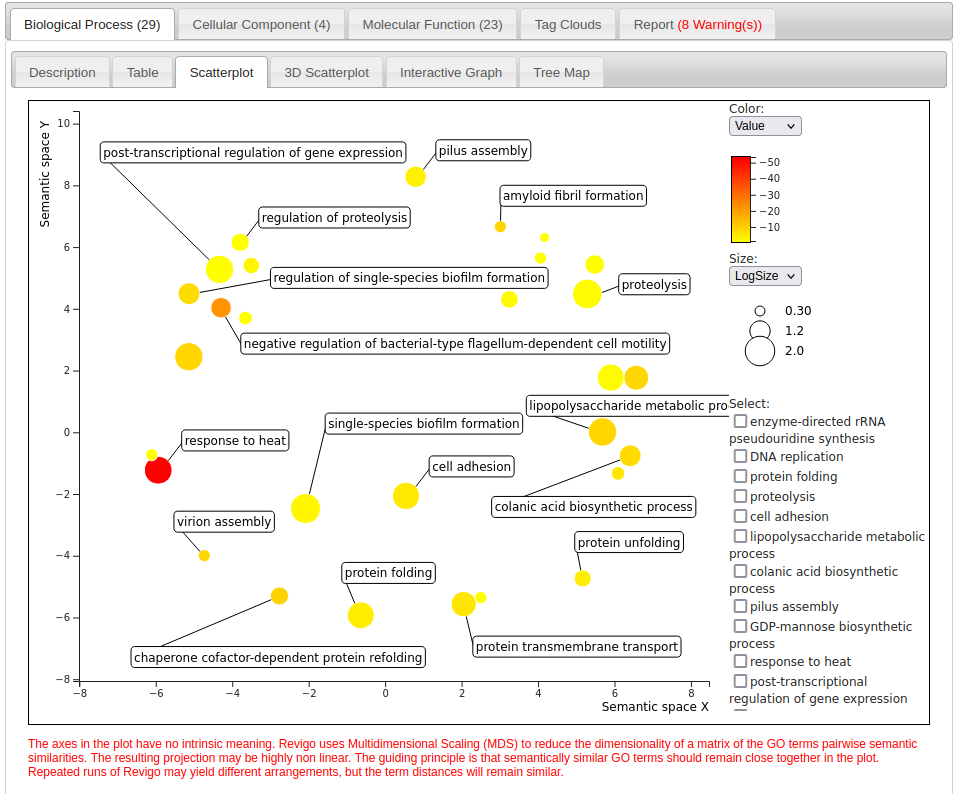
\includegraphics[width=16cm]{res.revigo.plot.png}    
  \label{fig:revigo1}
  \caption{Similarité sémantique des "GOTerm" - Processus biologiques - $\chi^2$ non ajustée  - set 6 - REVIGO} 
  \end{center}
  \end{figure} 
%%%%%%%%%%%%%%%%%%%%%%%%%%%%%%%%%%%%%%%%%%%% 

Les 4 termes impliqués dans la structure cellulaire sont : \textit{(cf. figure~\ref{fig:revigo2}}
\begin{itemize}
	\item membrane externe cellulaire
	\item pilus
	\item GroEL-ES complexe : protéines chaperonnes impliquée dans le repliement de nombreuses protéines \footnote{\url{https://fr.wikipedia.org/wiki/GroEL}}
	\item face externe de la membrane plasmique
\end{itemize}

 %%%%%%%%%%%%%%%%%%%%%%%%%%%%%%%%%%%%%%%%%%%%
  \begin{figure}[htbp] 
  \begin{center}
  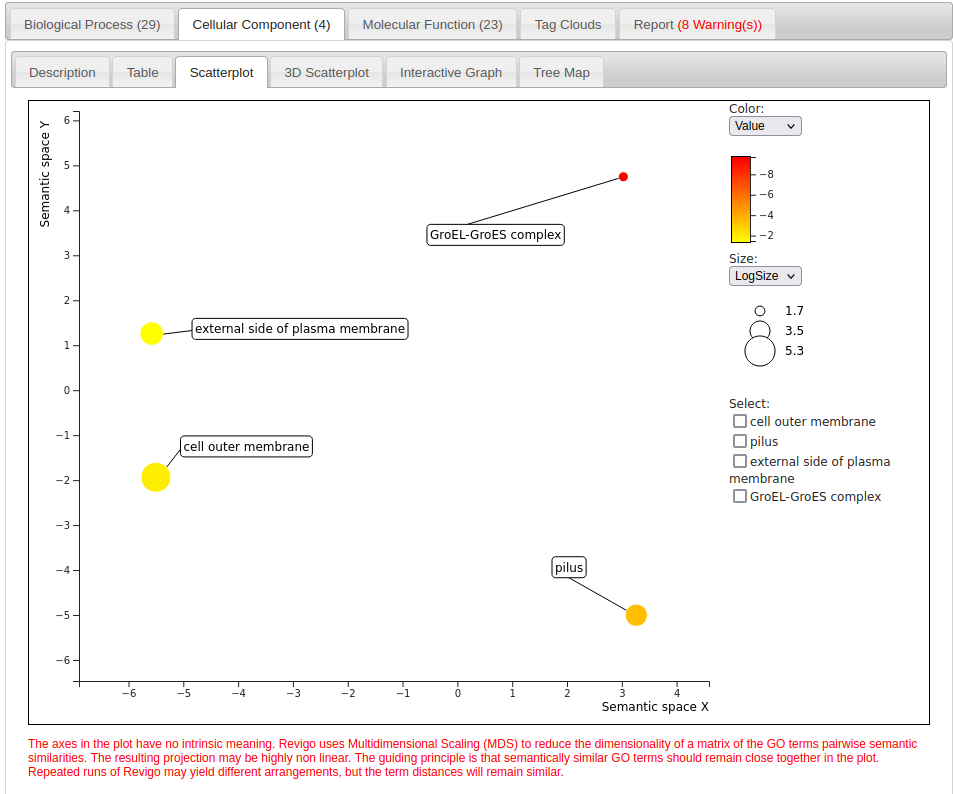
\includegraphics[width=16cm]{res.revigo.plot2.png}    
  \label{fig:revigo2}
  \caption{Similarité sémantique des "GOTerm" - Composants cellulaires - $\chi^2$ non ajustée  - set 6 - REVIGO} 
  \end{center}
  \end{figure} 
%%%%%%%%%%%%%%%%%%%%%%%%%%%%%%%%%%%%%%%%%%%% 


%%%%%%%%%%%%%%%%%%%%%%%%%%%%%%%%%%%%%%%%%%%%
  \begin{figure}[htbp] 
  \begin{center}
  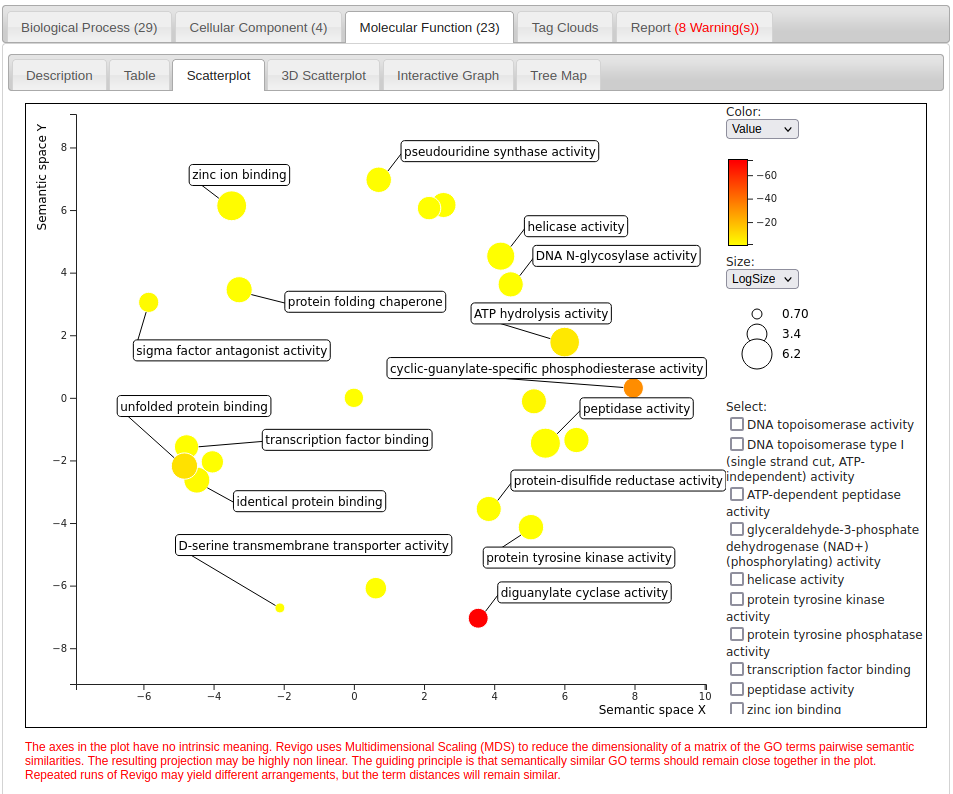
\includegraphics[width=16cm]{res.revigo.plot3.png}    
  \label{fig:revigo3}
  \caption{Similarité sémantique des "GOTerm" - Fonctions moléculaires- $\chi^2$ non ajustée  - set 6 - REVIGO} 
  \end{center}
  \end{figure} 
%%%%%%%%%%%%%%%%%%%%%%%%%%%%%%%%%%%%%%%%%%%% 
 
 
 Certains terme GO de la liste sont obsolètes, ou en doublons : \textit{(cf. figure~\ref{fig:warning}}
 %%%%%%%%%%%%%%%%%%%%%%%%%%%%%%%%%%%%%%%%%%%%
  \begin{figure}[htbp] 
  \begin{center}
  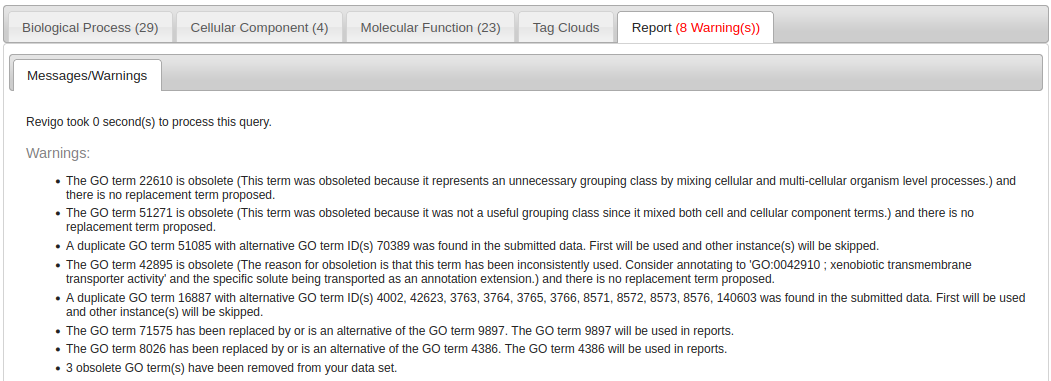
\includegraphics[width=16cm]{res.revigo.warning.png}    
  \label{fig:warning}
  \caption{Avertissement REVIGO $\chi^2$ non ajustée  - set 6 - REVIGO} 
  \end{center}
  \end{figure} 
%%%%%%%%%%%%%%%%%%%%%%%%%%%%%%%%%%%%%%%%%%%% 
 
 
%%%%%%%%%%%%%%%%%%%%%%%%%%%%%%%%%%%%%%%%%%%%
    




%%%%%%%%%%%%%%%%%%%%%%%%%%%%%%%%%%%%%%%%%%%%
\chapter{INTERPRETATION}
\thispagestyle{empty}
\clearpage
\newpage

Il semblerait que l'ensemble de gènes requêtes 6 code pour des protéines impliquées dans une réponse au stress. Cette réponse inclue :
\begin{itemize}
	\item la réception du signal (transduction sensorielle)
	\item la transmission du signal à la cellule (magnésium,transférase,protéines de liaison aux nucléotides,protéines chaperons,protéines de liaison à la GTP)
	\item et la réaction de défense (synthèse des exopolysaccharides, biosynthèse des Fimbrium) contre le stress occasionné.
\end{itemize}

La liste des termes de l'ontologie des gènes ("GOterm", base OBO) nous permet d'affiner l'hypothèse des fonctions biologiques des gènes inconnus. Il s'agirait de gènes impliquées dans une réponse à un stress thermique. La réponse au stress de la bactérie induit la création (ou le renforcement) du biofilm (processus de biosynthèse de l'acide colanique, activité phosphodiestérase spécifique du guanylate cyclique et diguanylate cyclase). La réponse au stress thermique semble inclure également :
 \begin{itemize}
\item  un changement biochimique de la membrane extérieure (biosynthèse de LPS, membrane externe bactérie Gram négative)
\item une réduction de la mobilité (régulation négative de la motilité cellulaire dépendante du flagelle de type bactérien)
\item renforcement de l'adhésion (création de firum)
\item protection des protéines (via chaperonnes, transformation du repliement de protéines)
\end{itemize}
D'après les données et les tests, il semblerait que la cellule bactérienne se prépare à affronter le stress en mettant en place une stratégie de défense plutôt que de fuite : perte de mobilité, changement de la structure de la membranne externe, renforcement du biofilm (bloc avec les bactéries voisines), création de fibrum qui renforce le phénomène d'adhésion (aux cellules eucaryotes de la paroi intestinal par exemple?) protection des protéines. Ces interprétations restent des hypothèses, à valider expérimentalement.
 (\textit{cf.~figure~\ref{fig:revigo1}})

%%%%%%%%%%%%%%%%%%%%%%%%%%%%%%%%%%%%%%%%%%%%
\section{[v2] VALIDATION ET COHÉSION DE COEXPRESSION}
%%%%%%%%%%%%%%%%%%%%%%%%%%%%%%%%%%%%%%%%%%%%

\textbf{Contrôle positif.} Pour vérifier que la méthode retrouve bien une biologie connue, nous l'appliquons à un cas d'école : l'opéron \textit{trp} (\textit{trpA--E}, b1260--b1264), cinq gènes qui synthétisent le L-tryptophane. L'outil retourne en tête la voie \texttt{TRPSYN-PWY} (\textit{L-tryptophan biosynthesis}, p = $2{,}1\times10^{-15}$, 5/5 gènes), suivie des superpathways des acides aminés aromatiques et du chorismate --- exactement la hiérarchie attendue, puisque le tryptophane dérive du chorismate. L'outil ne fait pas que « tourner », il \textbf{retrouve la bonne réponse} sur un cas de référence.

\textbf{Contrôle négatif.} Symétriquement, un ensemble de gènes \textit{tirés au hasard} ne devrait rien faire ressortir de significatif. Sur 200 tirages aléatoires de 113 gènes (même taille que le set d'étude), seuls 3\% produisent au moins une voie significative, soit en moyenne 0,05 terme par tirage --- à comparer aux 11 voies significatives du set 6. L'outil ne fabrique donc pas d'enrichissement à partir de bruit : le taux de faux positifs reste maîtrisé.

\textbf{Concordance avec un outil de référence.} Nous chiffrons l'accord avec l'application en ligne (silico.biotoul.fr/enrichment), prise comme étalon. Sur les termes GO du set 6, notre application retrouve \textbf{61\% des termes significatifs de l'étalon} (37 termes communs sur 61), mais en reporte beaucoup plus au total (270), ce qui donne un indice de Jaccard de 0,13. Cet écart ne traduit pas un désaccord sur la biologie mais notre \textbf{propagation des annotations le long de la hiérarchie GO} (règle du \textit{true-path} avec chemin de longueur variable) : les termes ancêtres, plus généraux, remontent aussi. C'est une limite méthodologique assumée (cf. section~\ref{sec:limites}), et non une erreur sur les fonctions identifiées.

\textbf{Exploitation des données STRING.} L'enrichissement indique \textit{pour quelles} fonctions un ensemble de gènes est annoté. Une question complémentaire, indépendante : ces gènes forment-ils réellement un \textbf{module} --- sont-ils plus coexprimés entre eux qu'un ensemble aléatoire de même taille ? Nous répondons par un test de permutation (2000 tirages) sur les arêtes de coexpression STRING, jusqu'ici seulement stockées dans la base.

\begin{table}[h]
\centering
\begin{tabular}{lcccc}
\hline
\textbf{Ensemble de gènes} & \textbf{gènes} & \textbf{force obs.} & \textbf{ratio vs aléatoire} & \textbf{p-value} \\
\hline
Set d'étude (query 6)   & 113 & 305\,975 & $\mathbf{13{,}2\times}$  & $\leq 5\times10^{-4}$ \\
Opéron \textit{trp} (contrôle) & 5 & 9\,934 & $\mathbf{252\times}$ & $\leq 5\times10^{-4}$ \\
\hline
\end{tabular}
\caption{Cohésion de coexpression (STRING) --- test de permutation. Le set d'étude est 13 fois plus coexprimé en interne que le hasard ; l'opéron \textit{trp}, co-transcrit par définition, atteint 252 fois (contrôle positif).}
\label{tab:coexpr}
\end{table}

\textbf{Deux angles convergents.} Nous disposons désormais de deux analyses \textit{indépendantes} qui pointent vers la même conclusion : (1) l'\textbf{enrichissement} (annotations) montre que ces gènes codent la biosynthèse de l'acide colanique et le programme biofilm ; (2) la \textbf{coexpression} (STRING) montre qu'ils forment un module réel ($13{,}2\times$ au-dessus du hasard), et non une liste arbitraire. La convergence de deux méthodes indépendantes renforce la confiance dans l'interprétation : d'après les données et les tests, le set 6 \textit{semblerait} être un module fonctionnel cohérent impliqué dans la réponse au stress et la formation du biofilm. Cette hypothèse resterait à confirmer expérimentalement.

%%%%%%%%%%%%%%%%%%%%%%%%%%%%%%%%%%%%%%%%%%%%
\section{[v2] LIMITES MÉTHODOLOGIQUES}
\label{sec:limites}
%%%%%%%%%%%%%%%%%%%%%%%%%%%%%%%%%%%%%%%%%%%%
\begin{itemize}
\item \textbf{Propagation GO (règle du \textit{true-path}).} Nous récupérons les GOTerm associés aux gènes \textit{ainsi que leurs ancêtres} (chemin \texttt{is\_a|part\_of|annotates*} de longueur variable). Les termes généraux (ex. \textit{metabolic process}) héritent donc de tous leurs descendants et ressortent quasi systématiquement : leurs p-valeurs ne sont pas directement interprétables. La concordance mesurée (61\% de recouvrement, Jaccard 0,13) quantifie ce phénomène. Une correction propre consisterait à tester chaque terme avec son ensemble de gènes réellement propagé et à ne pas confondre « enrichi » et « général » (approches conditionnelles de type \textit{elim}/\textit{weight}, cf. \texttt{topGO}).
\item \textbf{Non-indépendance des tests.} La correction de Benjamini-Hochberg suppose des tests approximativement indépendants. Or les termes GO sont emboîtés (parent/enfant) donc fortement corrélés : un terme et son parent ne constituent pas deux preuves indépendantes. Les q-valeurs rapportées doivent donc être lues comme des \textbf{bornes basses} (optimistes).
\item \textbf{Population de référence (« background »).} L'enrichissement est testé contre le génome entier (4315 gènes). Si l'ensemble requête provenait d'une expérience ne couvrant qu'une partie des gènes (puce, RNA-seq), le background correct serait la liste des gènes mesurés, pas la totalité du génome (cf. perspective en section Amélioration).
\end{itemize}

%%%%%%%%%%%%%%%%%%%%%%%%%%%%%%%%%%%%%%%%%%%%







%%%%%%%%%%%%%%%%%%%%%%%%%%%%%%%%%%%%%%%%%%%%
\chapter{CONCLUSION}
\thispagestyle{empty}
\clearpage
\newpage
\section{BIOLOGIQUE}
D'après les résultats d'enrichissement et de coexpression, l'ensemble de gènes 6 semblerait coder pour des protéines impliquées dans la réponse à un stress thermique, depuis la réception du signal (de stress) jusqu'à la cascade de réactions biochimiques et cellulaires qui en découle. Cette caractérisation est une hypothèse issue des données, qui resterait à confirmer expérimentalement. 

Cette approche bio-informatique, via la récolte des informations importantes pour un projet, leur organisation en BD sous forme de graphe (Avec Neo4j par exemple), et leur interrogation automatique via un programme (\textcolor{violet}{python}) est une formidable puissance pour analyser et caractériser une liste de gènes inconnus. Grâce à cette méthode, nous pouvons trouvé extrêmement facilement les fonctions biologiques et les publications associées. Par exemple, le travail de recherche de publication peut être très long et fastidieux. Cette méthode, permet vraiment de regrouper en un seul endroit, toutes informations relatives à un projet. \\ 
L'enjeu est de bien extraire les informations pertinentes (par exemple, il peut y avoir beaucoup de publication mentionnant chaque gène impliqué). Il s'agit d'une problématique classique dans bien des domaines, comment extraire le signal du bruit.

Il est important de fixer des limites raisonnables. Par exemple, à quel point est-il intéressant de poursuivre une étude qui possède un taux de recouvrement faible ?

\section{RETOUR CRITIQUES}

Nous n'avons pas intégré les "Alias" dans la base de donnée(nous nous en sommes rendue compte assez tardivement). \\
En comparant avec votre application (sur le site de silico.biotoul), nous ne trouvons pas les même résultats qu'avec la notre, qui semble être beaucoup moins restrictive. Néanmoins, les fonctions découvertes ne sont pas diamétralement opposées. \\

\section{AMÉLIORATION}
	\subsection{Application}
\begin{itemize}
\item L'application mérite une optimisation de la sortie. Il manquerait des graphiques de description des données, distributions (histogrammes, boîte à moustaches) par exemple 
\item Nous pourrions ajouté d'autres organismes afin de voir si les gènes sont conservés ou non
\item faire une analyse multivarié (ACP,regroupement des gènes, analyse discriminante), explorer les gènes co-exprimés
\item Nous avons vu l'approche par ensemble, mais nous pourrions utiliser une autre approche, basée sur des matrices de similarité (distance) et détecter des schémas de co-présence/co- exclusion\footnote{cf. partie 2 et 3 de \url{https://silico.biotoul.fr/enseignement/m2bbs/gdns-ap/GDNS-APG.Mise.en.oeuvre.html}}
\item \textbf{Population de référence (« background ») paramétrable.} Ici l'enrichissement est testé contre le génome entier (4315 gènes). Si l'ensemble requête provient d'une expérience ne couvrant qu'une partie des gènes (puce à ADN, RNA-seq), le background correct n'est pas le génome entier mais la liste des gènes réellement mesurés : les gènes non mesurés n'avaient aucune chance d'apparaître, et les inclure fausse les p-valeurs. Une option permettant de choisir le background (un sous-ensemble du génome plutôt que la totalité) rendrait l'outil directement applicable à des données de puce ou de RNA-seq.
\end{itemize}


	\subsection{Tests statistiques}
Le test de Fischer exact et le test du $\chi^2$ d’indépendance sont très souvent utilisées pour déceler une relation entre deux variables qualitative/binaire. Il s'agit de profils de présence/absence, c'est-à-dire des données binaires où chaque élément (gène, caractéristique, terme) est soit présent (1) ou absent (0). Néanmoins, il existe d'autres mesures de similarité que nous pourrions utiliser, comme par exemple : 

\begin{itemize}
\item \textbf{le test de McNemar : } Ce test est utilisé pour comparer des fréquences entre deux échantillons appariés. Le coefficient Q de Yule et les odd-ratio sont aussi des mesures d’associations entre données binaires (Tan et al., 2004).

\item \textbf{le test de Kruskal-Wallis : } test non paramétrique permettant de comparer plus de 2 échantillons et qui est en fait la généralisation du test de Mann-Whitney, mesure de l’association entre deux variables qualitatives 

\item \textbf{Coefficient de Jaccard : } couramment utilisé pour mesurer la similarité entre des ensembles binaires. Il est particulièrement adapté aux profils de présence/absence. Il mesure la proportion d'éléments en commun entre deux ensembles par rapport à la taille totale de leurs éléments

\item \textbf{Distance de Hamming : } calcule le nombre de positions à partir desquelles deux profils binaires diffèrent. Plus les profils diffèrent, plus la distance de Hamming est élevée.

\item \textbf{Coefficient de Dice : } similaire au coefficient de Jaccard et est également utilisé pour mesurer la similarité entre deux ensembles binaires. 
\end{itemize}

Le coefficient de Jaccard est souvent utilisé pour des ensembles de grande taille, tandis que la distance de Hamming peut être appropriée si vous souhaitez mesurer la différence exacte entre deux profils. 

Il est recommandé de tester plusieurs mesures de similarité et de choisir celle qui semble la plus pertinente pour chaque analyse en fonction des besoins et de la nature des données.


J'aurai peut être vu un test d'adéquation du  $\chi^2$ pour suivre la logique des 2 tests que nous avons réalisé ('binomial' et 'hypergeometric'). De plus, peut être que nous pourrions tester une autre stratégie pour ajuster les p-valeurs si multi-test (FDR).

\paragraph{[v2] En synthèse --- deux priorités.} Parmi les pistes ci-dessus, deux me paraissent prioritaires car elles corrigent des limites réelles de l'analyse (cf. section~\ref{sec:limites}), plutôt que d'ajouter des mesures pour le plaisir :
\begin{enumerate}
\item \textbf{Un test GO conditionnel} (type \textit{elim}/\textit{weight}, cf. \texttt{topGO}) pour traiter la non-indépendance des termes emboîtés et éviter que les termes généraux ne dominent --- c'est la correction directe du biais \textit{true-path} mesuré par la concordance.
\item \textbf{Un background paramétrable} pour que l'enrichissement reste valide quand l'ensemble requête provient d'une expérience à couverture partielle (puce, RNA-seq).
\end{enumerate}
Les autres mesures (Jaccard, Hamming, Dice, McNemar, Kruskal-Wallis) relèvent d'une approche par matrices de similarité, intéressante mais distincte de l'approche par enrichissement retenue ici.

\section{BILAN PERSONNEL}
J'ai vraiment adoré ce projet, notamment les aspects suivant :
\begin{itemize}
	\item comment collecter et où aller chercher les informations importantes
	\item avoir été sensibilisée aux problèmes d'identifiants, de références différents selon les sources de données et comment faire le lien entre eux
	\item comment créer une base de données interactive
	\item comment relier les informations entre elles, et avec des requêtes pouvoir répondre à des questions où il aurait fallu des heures si fait manuellement
	\item en connectant ainsi les données, voir des connexions entre les événements pas si évident au premier abort
\end{itemize}
J'aime beaucoup le principe d'organiser les données en graphe, plus en adéquation avec ma façon de voir les choses, plutôt que linéairement. J'ai entrevu des répercussions dans les futurs projets en biologie notamment, et j'ai hâte de réappliquer cette méthode à d'autres problématiques. \\
J'ai aimé programmer l'application python qui permet d'automatiser des demandes classiques
à partir d'une liste de gènes d’intérêts. Super exemple de ce que nous pouvons faire avec python. Même si la mise en place est longue, le gain de temps sur le long terme est indéniable.\\
Je suis très reconnaissante à mes camarades de classe Margaux DORE, Han PHAN et Claire D. pour l'étroite entraide entre nous, complètement indispensable. Nous avons continué Claire et moi de créer la base de donnée et l'application ensemble. Ce projet était très long, et au premier abord complexe, car beaucoup de notions à intégrer d'un coup. Le fait d'échanger et de travailler en équipe (équilibrée et dans la bonne humeur) avec Claire,  nous a permis clairement (sans jeu de mot) de mieux comprendre l'ensemble. C'est définitivement un projet à faire à plusieurs ! 
La difficulté pour moi a été de savoir quand s'arrêter ! Beaucoup de questions, de choses à tester, et j'ai une certaine tendance à me laisser entraîner par ma curiosité. J'ai eu l'impression juste d'à peine ouvrir une porte sur de vastes possibilités. \\
\textbf{Bilan : } projet top, mais longgggg !! A proposer à faire en groupe, du moins pour la partie construction BD et application, je pense :) \\
Merci pour tout !


\begin{tikzpicture}[remember picture, overlay]
 \begin{scope}[shift={(current page.south east)},shift={(-3,3)},scale=1]
 \shade[ball color=blue,opacity=.6] (0,0) circle (10ex);
 \shade[ball color=blue,opacity=.8] (-1.7,1) circle (5ex);
 \shade[ball color=blue,opacity=.8] (-1.5,3) circle (2ex);
 \shade[ball color=blue,opacity=.5] (0.5,3) circle (1ex);
 \shade[ball color=blue,opacity=.8] (-1,4) circle (1ex);
 \shade[ball color=blue,opacity=.6] (-3.5,2.5) circle (2ex);
 \shade[ball color=blue,opacity=.8] (-2.5,4.5) circle (4ex);
 \shade[ball color=blue,opacity=.5] (-3,4) circle (3ex);
 \shade[ball color=blue,opacity=.8] (-4.5,4.5) circle (3ex);
 \shade[ball color=blue,opacity=.5] (-5.1,4.7) circle (2ex);
 \shade[ball color=blue,opacity=.8] (-5,6) circle (1.5ex);
 \shade[ball color=blue,opacity=.6] (-3.5,5.5) circle (2ex);
 \shade[ball color=blue,opacity=.8] (-5,3) circle (1ex);
 \end{scope}
\end{tikzpicture}
%%%%%%%%%%%%%%%%%%%%%%%%%%%%%%%%%%%%%%%%%%%%





%%%%%%%%%%%%%%%%%%%%%%%%%%%%%%%%%%%%%%%%%%%%
\chapter{ANNEXE - SCRIPT R1 - TRANSFORMATION DONNÉES}
\newpage
\label{annexe:R1}
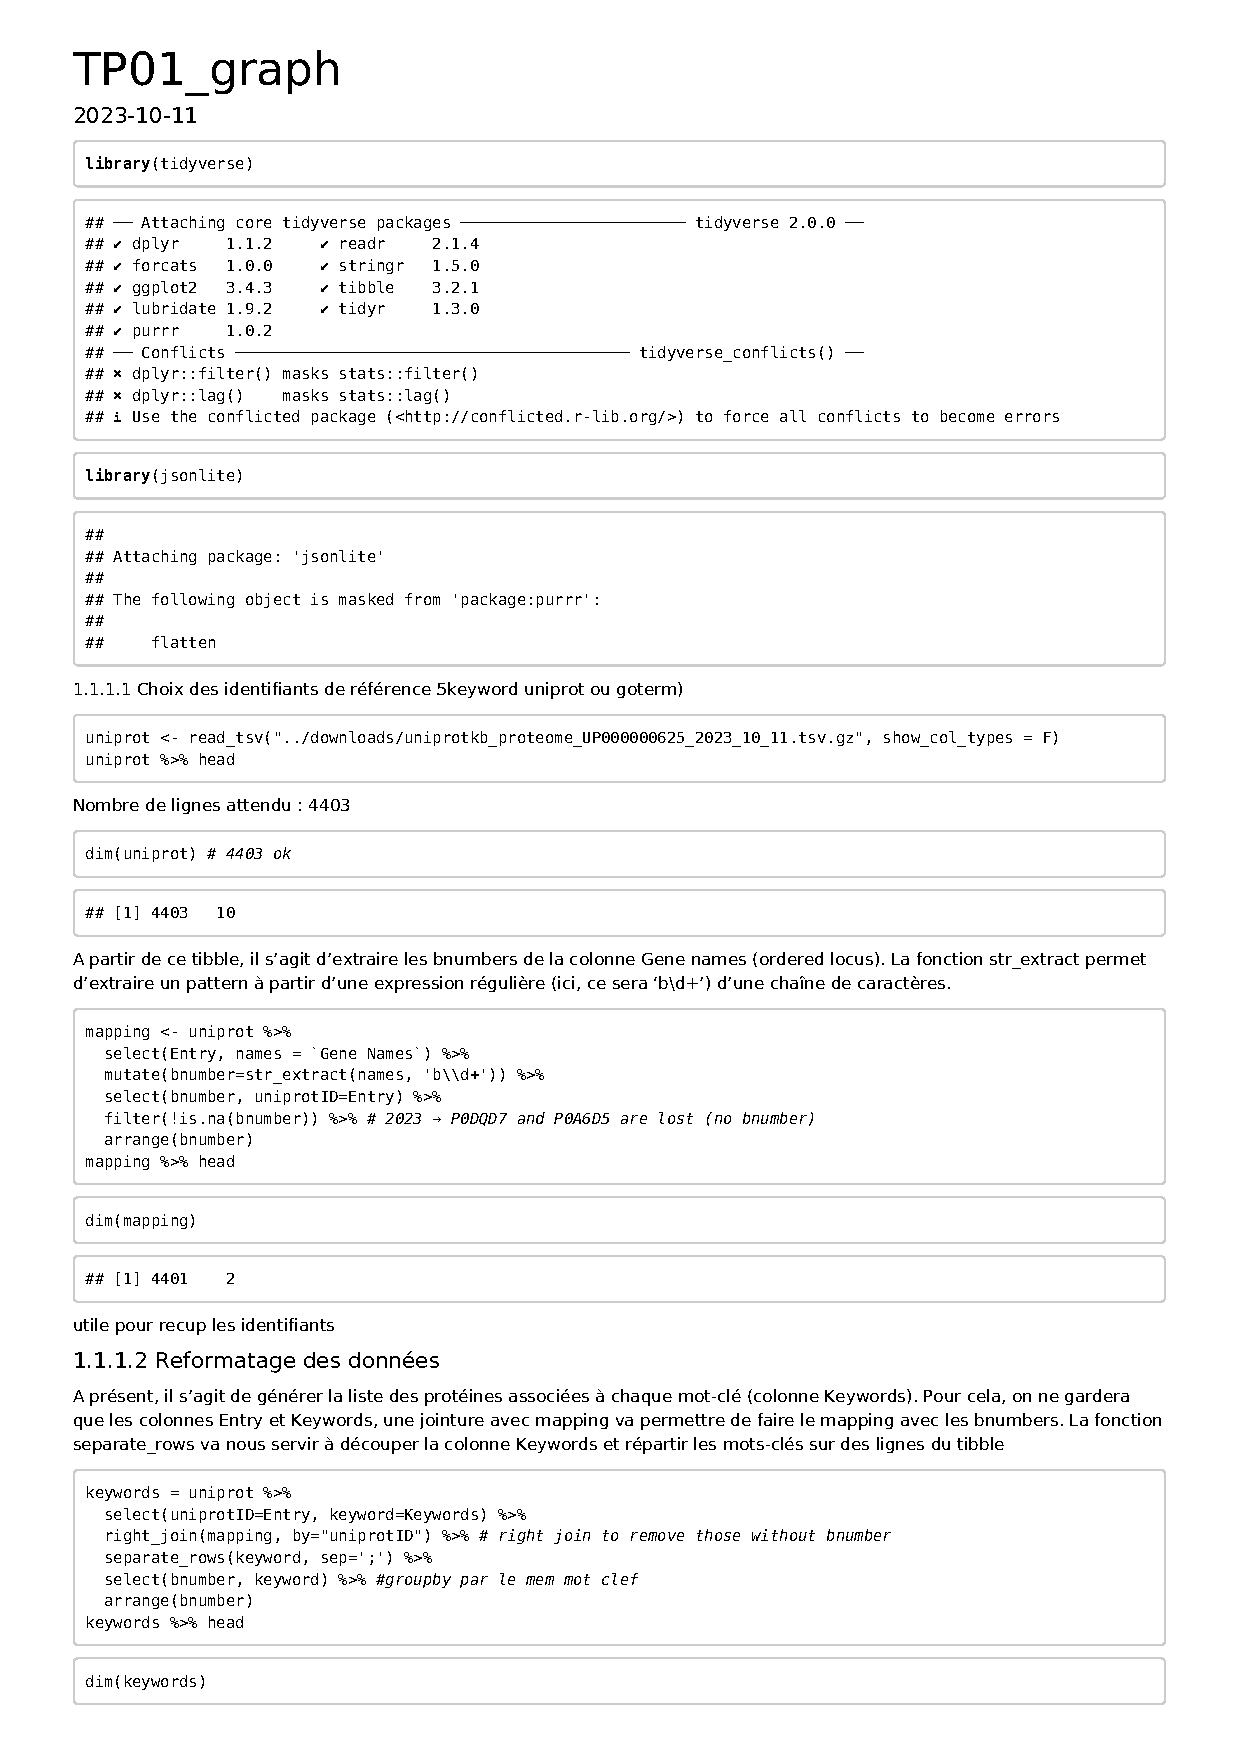
\includepdf[pages=-]{R1.pdf} 
%%%%%%%%%%%%%%%%%%%%%%%%%%%%%%%%%%%%%%%%%%%%





%%%%%%%%%%%%%%%%%%%%%%%%%%%%%%%%%%%%%%%%%%%%
\chapter{ANNEXE - SCRIPT R2 - INTEGRATION DES FICHIERS CSV DANS LA BASE DE DONNÉES NEO4J}
\newpage
\label{annexe:R2}
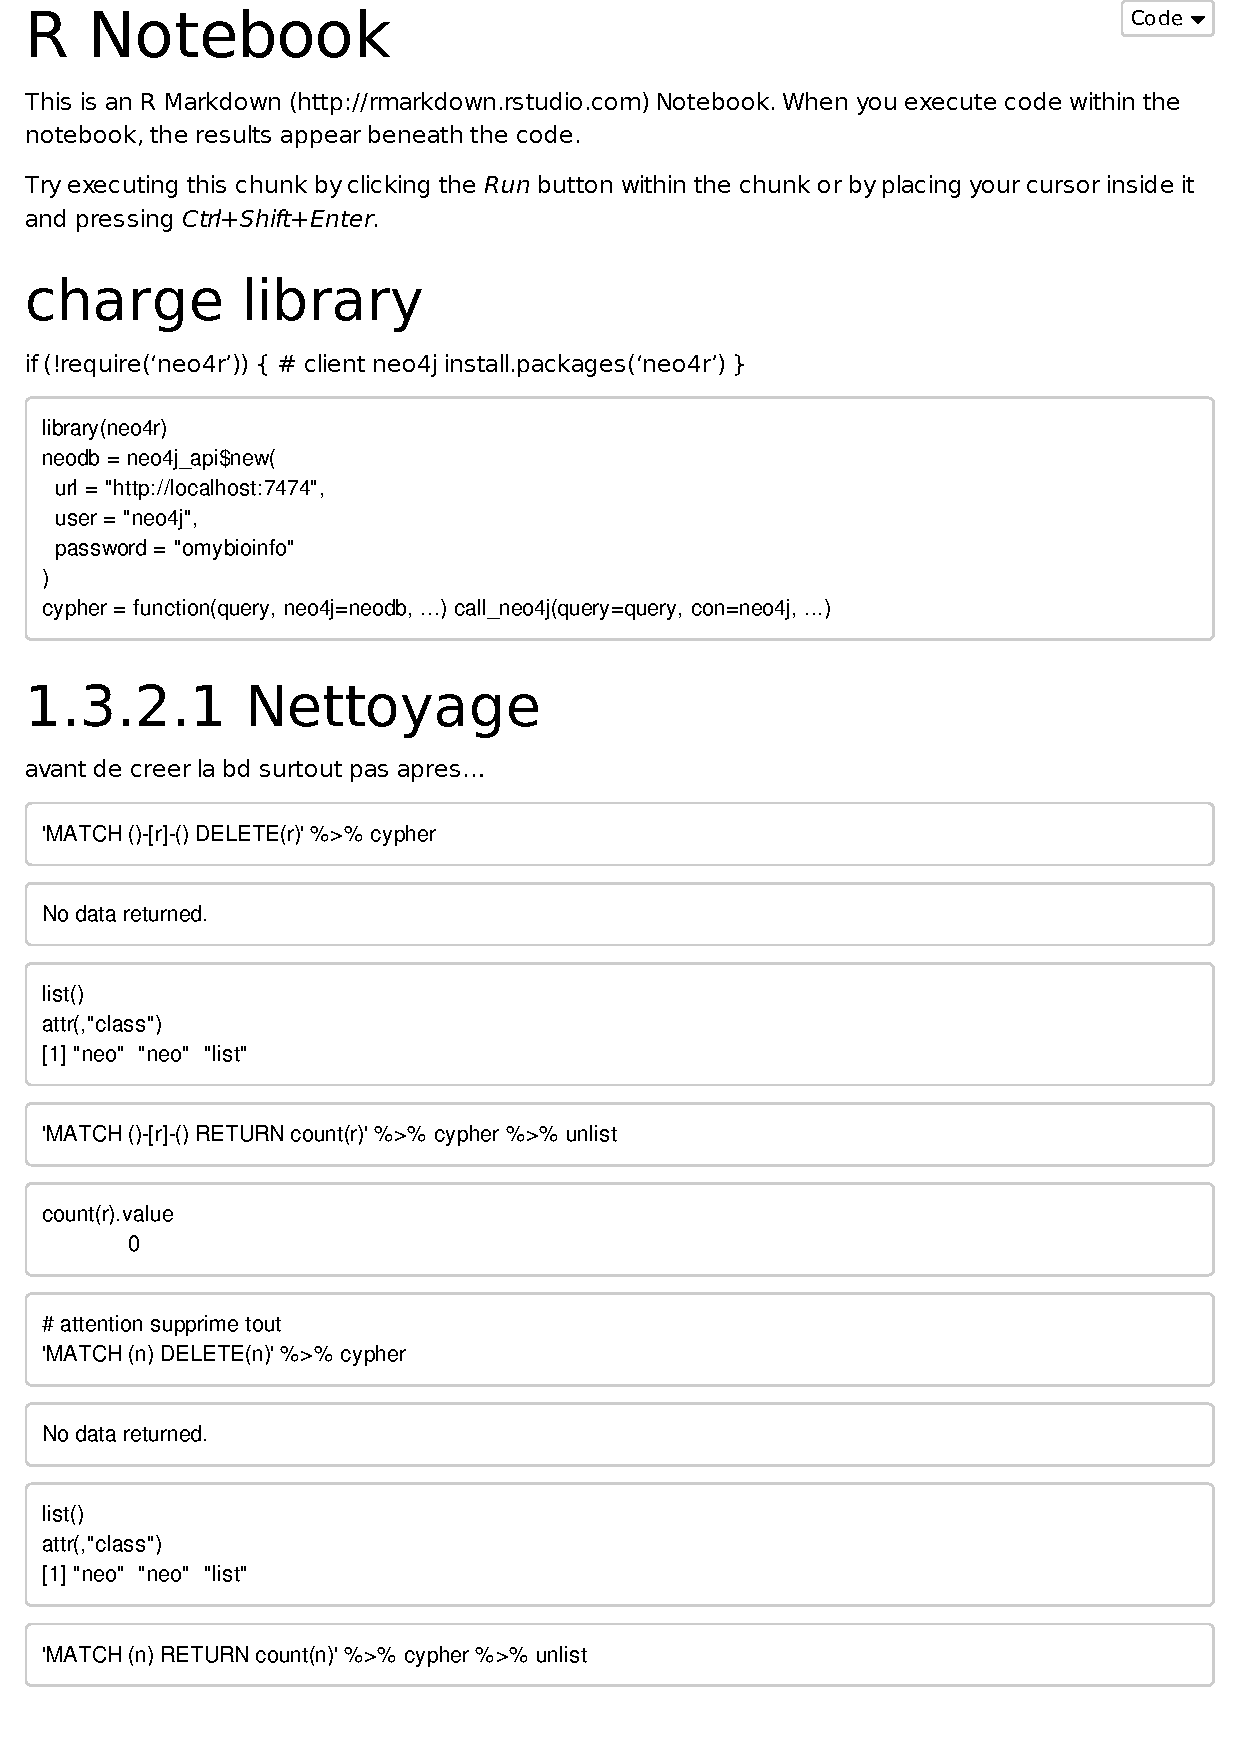
\includepdf[pages=-]{R2.pdf} 
%%%%%%%%%%%%%%%%%%%%%%%%%%%%%%%%%%%%%%%%%%%%





%%%%%%%%%%%%%%%%%%%%%%%%%%%%%%%%%%%%%%%%%%%%
\chapter{ANNEXE - SCRIPT PYTHON - APPLICATION ENRICHISSEMENT}
\newpage
\label{annexe:app}

\begin{verbatim}
#!/bin/env python
# conda install python3 biopython requests
# ./gbff.to.bnumber.GeneID.py > mapping.bnumber_ncbi.tsv

# UPLOAD PACKAGES
from py2neo import * # conda install py2neo, monotonic
from py2neo.matching import *
import argparse
from pprint import pprint
from os.path import isfile
import json
from scipy.stats import binom, hypergeom, chi2_contingency  # pip install scipy


# CONNECTION TO NEO4J
neo = Graph("bolt://localhost:7687",
            auth=("neo4j","omybioinfo"))
nodes = NodeMatcher(neo)
 

# SCRIPT PARAMETERS #######################################################
parser = argparse.ArgumentParser(description='Search enriched terms/categories 
in the provided (gene) set')
parser.add_argument('-q', '--query', required=True, 
help='Query set (gene nodes in Neo4j).')
parser.add_argument('-t', '--type', required=True, choices=['Keyword', 'Pathway','TU','GOTerm','InterPro','PubMed'], help='Type of target sets: keyword, pathway,TU,GOterm,Interpro,pubmed')
parser.add_argument('-a', '--alpha', required=False, type=float, default=0.05, 
help='Significance threshold.')
parser.add_argument('-c', '--adjust', required=False, action="store_true", 
help='Adjust for multiple testing (FDR).')
parser.add_argument('-m', '--measure', required=False, default='binomial', 
help='Dissimilarity index: binomial (default), hypergeometric, chi2 or coverage')
parser.add_argument('-l', '--limit', required=False, type=int, default=0, 
help='Maximum number of results to report.')
parser.add_argument('-v', '--verbose', required=False, action="store_true", help='Talk a lot.')
param = parser.parse_args()


# Path Query
path = '../query/query6.txt'


# LOAD QUERY #######################################################################
text = param.query
query = set()
if isfile(text):
    with open(text) as f:
        content = ' '.join(f.read().split('\n')).split()
        query |= set(content)
else: # parse string
    query |= set(text.split())

if param.verbose:
  print(f'query set: {query}')

# LOAD TARGET/REFERENCE SETS #######################################################
population = nodes.match("Gene")
pprint(population)

# POPULATION SIZE = total number of genes in the database
n_gene_total = population.count() # len(population)
pprint(f"population size: {n_gene_total}")

# QUERY SIZE = number of genes in the query
query_size = len(query)
pprint(f"Number of genes in the query: {query_size}")

# EXTRACT query genes from the database:

target = param.type
if target == 'Keyword': # if we want to search for keywords
    cypher = f"MATCH (k:{target})-->(g:Gene) WHERE g.id IN {list(query)} 
    RETURN DISTINCT k"
    res = neo.run(cypher)#.to_table()

elif target == 'GOTerm': # EXTRACT GO TERMS FROM query genes from the database:
    cypher = f"MATCH (k:{target})-[:is_a|part_of|annotates*]->(g:Gene) 
    WHERE g.id IN {list(query)} RETURN DISTINCT k.id, k.desc" 
    
    res = neo.run(cypher).to_table()

elif target == 'TU': # EXTRACT TU FROM query genes from the database:
    cypher = f"MATCH (k:{target})-[:harbors]->(g:Gene) WHERE g.id 
    IN {list(query)} RETURN DISTINCT k.id, k.desc" 
    res = neo.run(cypher).to_table()

elif target == 'Pathway': # EXTRACT PATHWAY FROM query genes from the database:
    cypher = f"MATCH (k:{target})-[:requires]->(g:Gene) WHERE g.id 
    IN {list(query)} RETURN DISTINCT k.id, k.desc" 
    res = neo.run(cypher).to_table()

elif target == 'InterPro': # EXTRACT Interpro FROM query genes from the database:
    cypher = f"MATCH (k:{target})-[:encoded_in]->(g:Gene) WHERE g.id 
    IN {list(query)} RETURN DISTINCT k.id" 
    res = neo.run(cypher).to_table()

elif target == 'PubMed': # EXTRACT PubMed FROM query genes from the database:
    cypher = f"MATCH (k:{target})-[:cites]->(g:Gene) WHERE g.id 
    IN {list(query)} RETURN DISTINCT k.id" 
    res = neo.run(cypher).to_table()

if param.verbose:
    pprint(f'Cyper request: {cypher}')
    pprint(f'target set: {res}')


#  STATISTICAL TESTS #######################################################################
results = [] 
liste_proba = [] # list of dictionaries to store results (probabilities)
dico_proba = {}
desc = []
for r in res:
    # EXTRACT GENES ASSOCIATED (bnumber) WITH CYPHER REQUESTS
    if target == 'Keyword':
        set_id = r['k']['id']
        cypher2 = f"MATCH (t:{target})-->(g:Gene) WHERE t.id = '{set_id}' 
        RETURN DISTINCT g.id" 
    elif target == 'GOTerm':   
        set_id = r[0] 
        desc = r[1]
        cypher2 = f"MATCH (t:{target})-[:is_a|part_of|annotates*]->(g:Gene) 
        WHERE t.id = '{set_id}' RETURN DISTINCT g.id"
    elif target == 'TU':   
        set_id = r[0] 
        desc = r[1]
        cypher2 = f"MATCH (t:{target})-[:harbors]->(g:Gene) WHERE t.id = '{set_id}' 
        RETURN DISTINCT g.id"
    elif target == 'Pathway':   
        set_id = r[0] 
        desc = r[1]
        cypher2 = f"MATCH (t:{target})-[:requires]->(g:Gene) WHERE t.id = '{set_id}' 
        RETURN DISTINCT g.id"    
    elif target == 'InterPro':   
        set_id = r[0] 
        cypher2 = f"MATCH (t:{target})-[:encoded_in]->(g:Gene) WHERE t.id = '{set_id}' 
        RETURN DISTINCT g.id"    
    elif target == 'PubMed':   
        set_id = r[0] 
        cypher2 = f"MATCH (t:{target})-[:cites]->(g:Gene) WHERE t.id = '{set_id}' 
        RETURN DISTINCT g.id"    
    
    # EXECUTE CYPHER REQUESTS ACCORDING TO THE TARGET TYPE
    result2 = neo.run(cypher2)
    
    # EXTRACT UNIQUE GENES ASSOCIATED WITH CYPHER REQUESTS
    elements = set(i[0] for i in result2.to_table()) 
    common_elements = elements.intersection(query)  # common elements between query and target
    k = len(common_elements) # c/k:number of successes in the population = common between query and elements
    t = len(elements)
    p = len(elements)/n_gene_total # proba of success each essay

    # COVERAGE ####################################################
    if param.measure == 'coverage':
        proba = 1 - (k/query_size) * (k/t)

    # BINOMIAL TEST ####################################################
    if param.measure == 'binomial': 
        # based on success
        # proba = 1 - binom.cdf(len(common_elements)-1, query_size, p) #query_size - len(common_elements)
        # based on failure : best
        proba = binom.cdf(query_size - k, query_size, 1 - p)

    # HYPERGEOMETRIC TEST ##################################################
    if param.measure == 'hypergeometric':
        proba = 1 - hypergeom.cdf(k - 1, n_gene_total, t, query_size)
        # x = k, M = n_gene_total, t = len(elements), n = query_size 
        # pdf = hypergeom.pmf(x, M, n, N)
        # k success parmi n du query/target, N = population size, 
        #t = number of target in the population, N = number of query

    # CHI2 ########################################################
    if param.measure == 'chi2': # adjusted chi square cdf(x, df, loc=0, scale=1)
        # Creation of the contingency table as observed = [[c, q - c], [t - c, g - q - t + c]]
        observed = [[k, query_size - k], [ t - k, n_gene_total - ( t + query_size - k)]]
        # chi2_contingency test
        chi2_stat, proba, _, _ = chi2_contingency(observed)


    # if proba <= param.alpha:
    dico_proba = {
                  "id": set_id, 
                  "p-value": proba,
                  'common.n':len(common_elements), 
                  'target.n': len(elements),
                  'elements.target': elements, 
                  'elements.common': common_elements,
                  'desc': desc
                }      
    liste_proba.append(dico_proba)
    
liste_triee = sorted(liste_proba, key=lambda x: x["p-value"])

if param.adjust:
    liste_ajust = []
    
    for i, r in enumerate(liste_triee):
        p_val_ajust = (r["p-value"] * len(liste_triee)) / (i + 1)  # [v2] m = nb de tests, pas query_size
        if p_val_ajust <= param.alpha:
            liste_ajust.append(r)
            
    pprint(f'Number of significative adjusted p-value(0.05): {len(liste_ajust)}')
    for r in liste_ajust:
        print("{}\t{}\t{}/{}\t{}\t{}".format(r['id'], r['p-value'], 
        r['common.n'], r['target.n'], r['desc'], ', '.join(r['elements.common'])))

else:
    pprint(f'Number of significative adjusted p-value(0.05): {len(liste_triee)}')
    for r in liste_triee:
        print("{}\t{}\t{}/{}\t{}\t{}".format(r['id'], r['p-value'], 
        r['common.n'], r['target.n'], r['desc'], ', '.join(r['elements.common'])))
\end{verbatim}
%%%%%%%%%%%%%%%%%%%%%%%%%%%%%%%%%%%%%%%%%%%%

%%%%%%%%%%%%%%%%%%%%%%%%%%%%%%%%%%%%%%%%%%%%
\chapter{ANNEXE - ENSEMBLE QUERY 6 - set.6.M2.txt}
\newpage
\label{annexe:Q6}

b0014 b0015 b0058 b0210 b0315 b0385 b0438 b0439 b0457 b0473 b0492 b0631 b0660 b0833 b0834 b0879 b0966 b1025 b1037 b1038 b1039 b1040 b1041 b1042 b1043 b1060 b1114 b1163 b1168 b1274 b1279 b1280 b1285 b1321 b1322 b1341 b1341 b1379 b1380 b1489 b1490 b1522 b1535 b1664 b1707 b1779 b1785 b1786 b1794 b1815 b1829 b1956 b2044 b2045 b2046 b2047 b2048 b2049 b2050 b2051 b2052 b2053 b2054 b2055 b2056 b2057 b2058 b2059 b2060 b2061 b2062 b2067 b2176 b2395 b2503 b2592 b2603 b2604 b2614 b3178 b3179 b3252 b3279 b3400 b3401 b3461 b3497 b3498 b3525 b3529 b3594 b3635 b3686 b3687 b3931 b3932 b3989 b4061 b4140 b4142 b4143 b4174 b4175 b4208 b4312 b4313 b4314 b4315 b4316 b4317 b4318 b4319 b4320 b4484 
%%%%%%%%%%%%%%%%%%%%%%%%%%%%%%%%%%%%%%%%%%%%



\end{document}